\chapter{Experimental Evaluation}
\label{sec:experiental_evaluation}

file = content/chapters/chapter5.tex


\section{Experimental Setup and Dataset}


\subsection{Experimental Protocol}
\label{subsec:experimental_protocol}

The experiments were conducted using the eye-in-hand calibration system described in Chapter~\ref{sec:system_architecture}. The FANUC LR Mate 200iD manipulator carried the Cognex industrial camera while a rigid ChArUco board remained fixed within the robot workspace. At each acquisition pose, the robot was manually positioned using the teach pendant, an image of the calibration target was captured, and the corresponding robot pose was recorded by the controller. The resulting image--pose pairs constituted the input dataset used throughout the experimental evaluation.

\paragraph{Pose acquisition strategy}
The selection of robot configurations was performed manually in order to ensure a sufficiently rich and well-conditioned dataset for calibration. In particular, the acquisition strategy was designed according to the following criteria:

\begin{itemize}
	\item \textbf{Large rotational diversity:} robot orientations were varied across multiple axes to ensure observability of the full 6D pose space.
	
	\item \textbf{Varied viewing angles:} the calibration target was observed from significantly different perspectives, avoiding near-constant viewpoints.
	
	\item \textbf{Consistent target visibility:} the ChArUco board was kept fully or mostly visible in the camera field of view at each pose to guarantee reliable feature detection.
	
	\item \textbf{Avoidance of degenerate motions:} purely translational motions or near-constant orientations were intentionally avoided, as they can lead to poorly conditioned hand-eye calibration problems.
	
	\item \textbf{Workspace coverage:} poses were distributed across the reachable workspace of the robot in order to improve numerical stability and reduce bias in the estimated transformation.

	
\end{itemize}

Overall, this strategy aimed at balancing practical acquisition constraints with the observability requirements of the hand-eye calibration problem.

\paragraph{Acquisition overview}
Figure~\ref{fig:dataset_viewpoints} illustrates representative viewpoints collected during the acquisition process, highlighting the variability in camera orientation and position relative to the calibration target.

\begin{figure}[htbp]
	\centering
	
	
	% --- Placeholder subfigure 1 ---
	\begin{subfigure}[t]{0.48\textwidth}
		\centering
		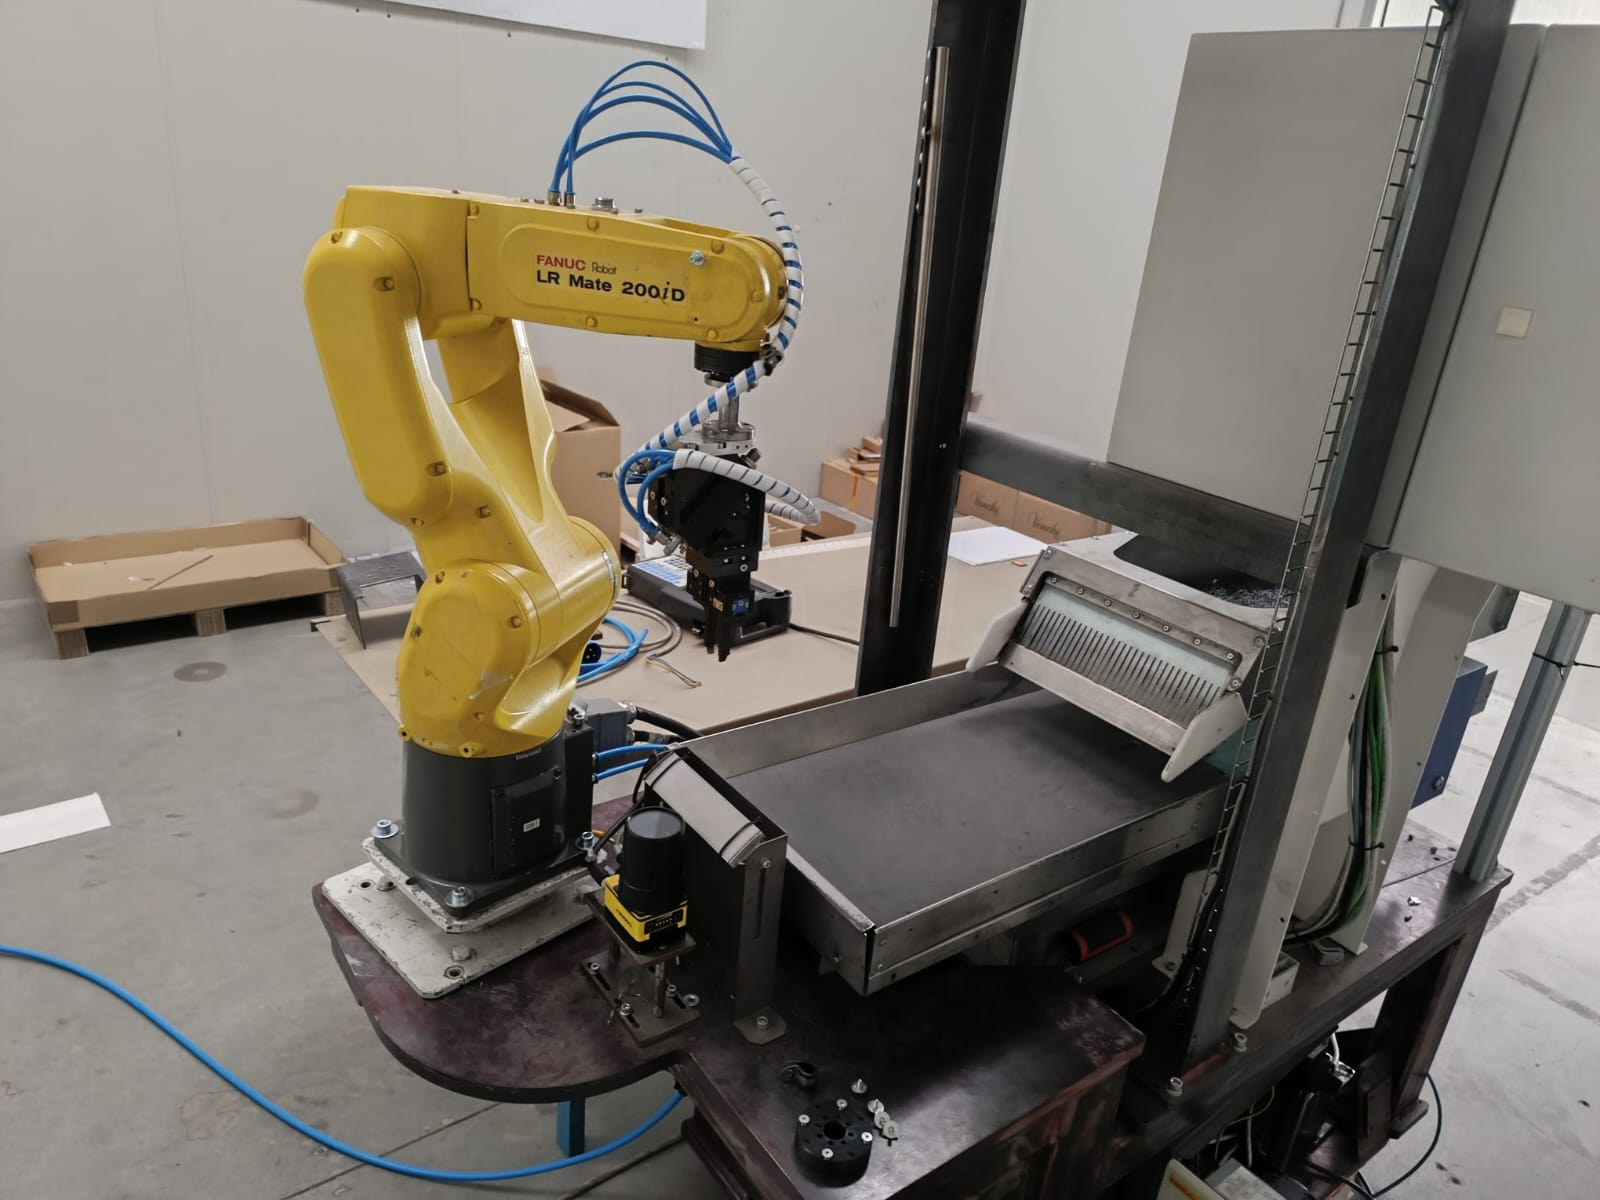
\includegraphics[width=\textwidth]{images/chapter5Images/workspace.png}
		\caption{Full experimental workspace, ChArUco board placed inside container.}
		\label{fig:workspace_view}
	\end{subfigure}
	\hfill
	% --- Placeholder subfigure 2 ---
	\begin{subfigure}[t]{0.48\textwidth}
		\centering
		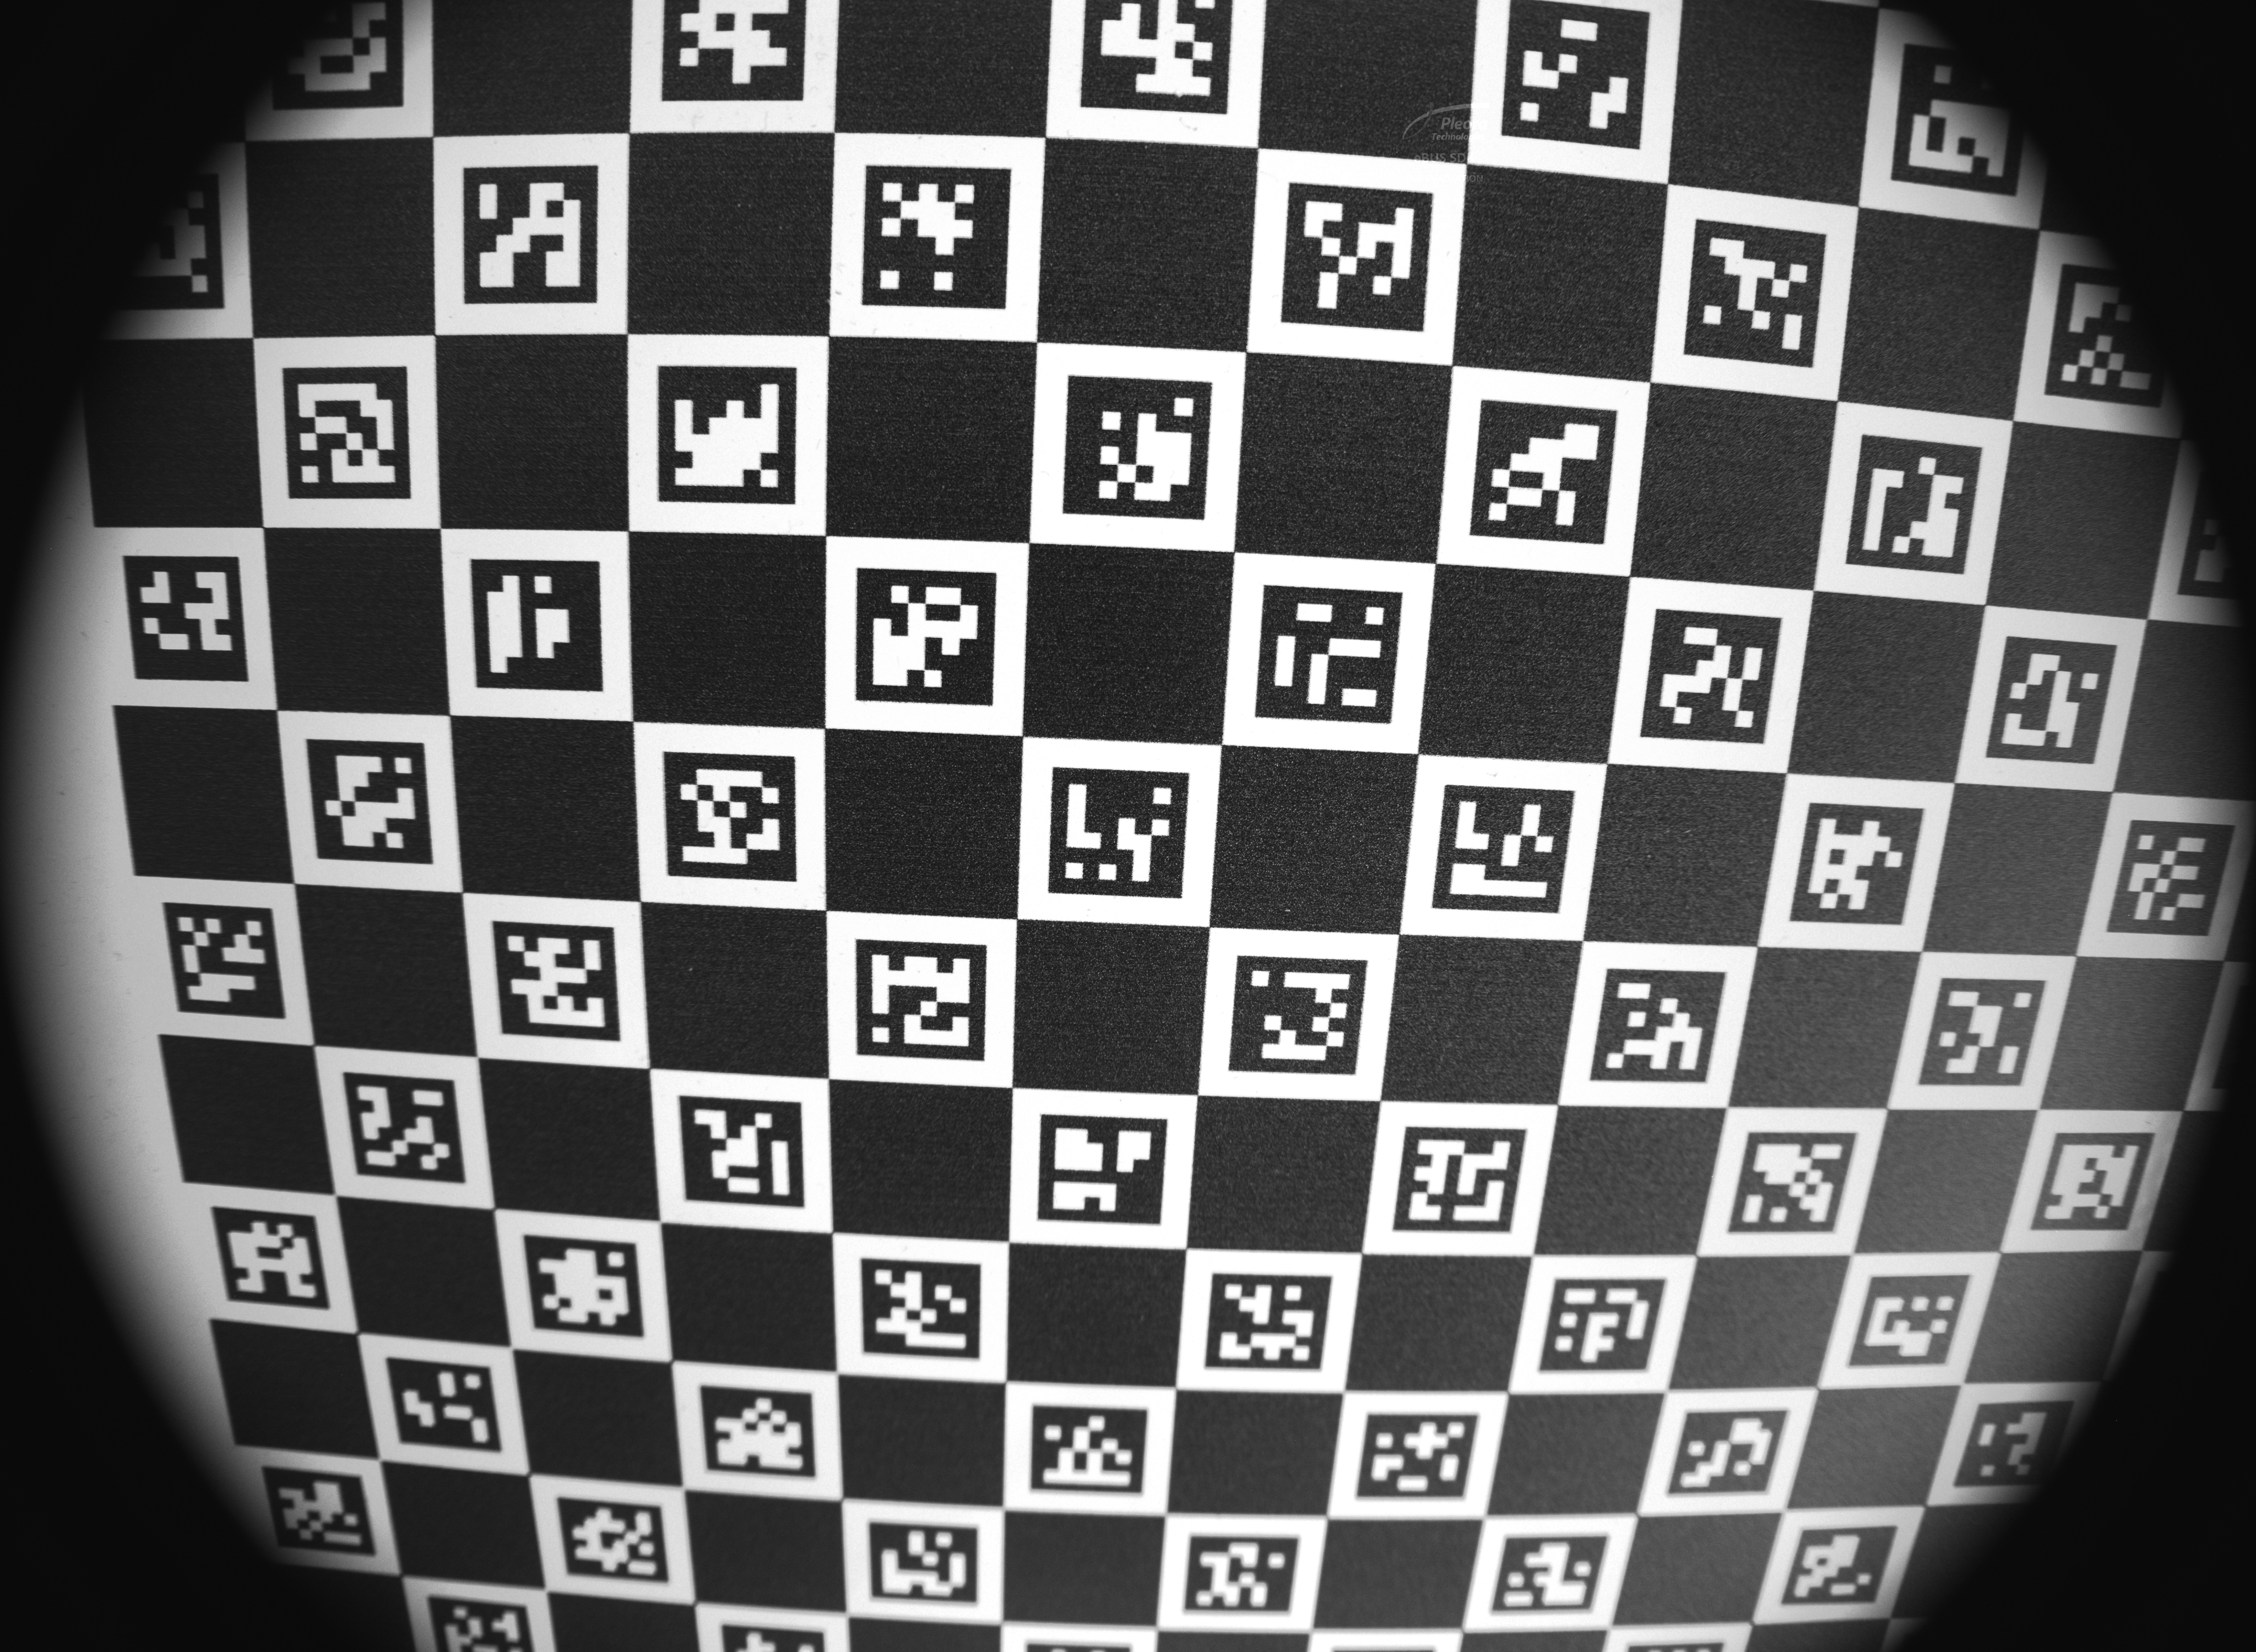
\includegraphics[width=\textwidth]{images/chapter5Images/006.png}
		\caption{Example of an acquired viewpoint with moderate viewing angle.}
		\label{fig:viewpoint_1}
	\end{subfigure}
	
	\vspace{0.5cm}
	
	% --- Placeholder subfigure 3 ---
	\begin{subfigure}[t]{0.48\textwidth}
		\centering
		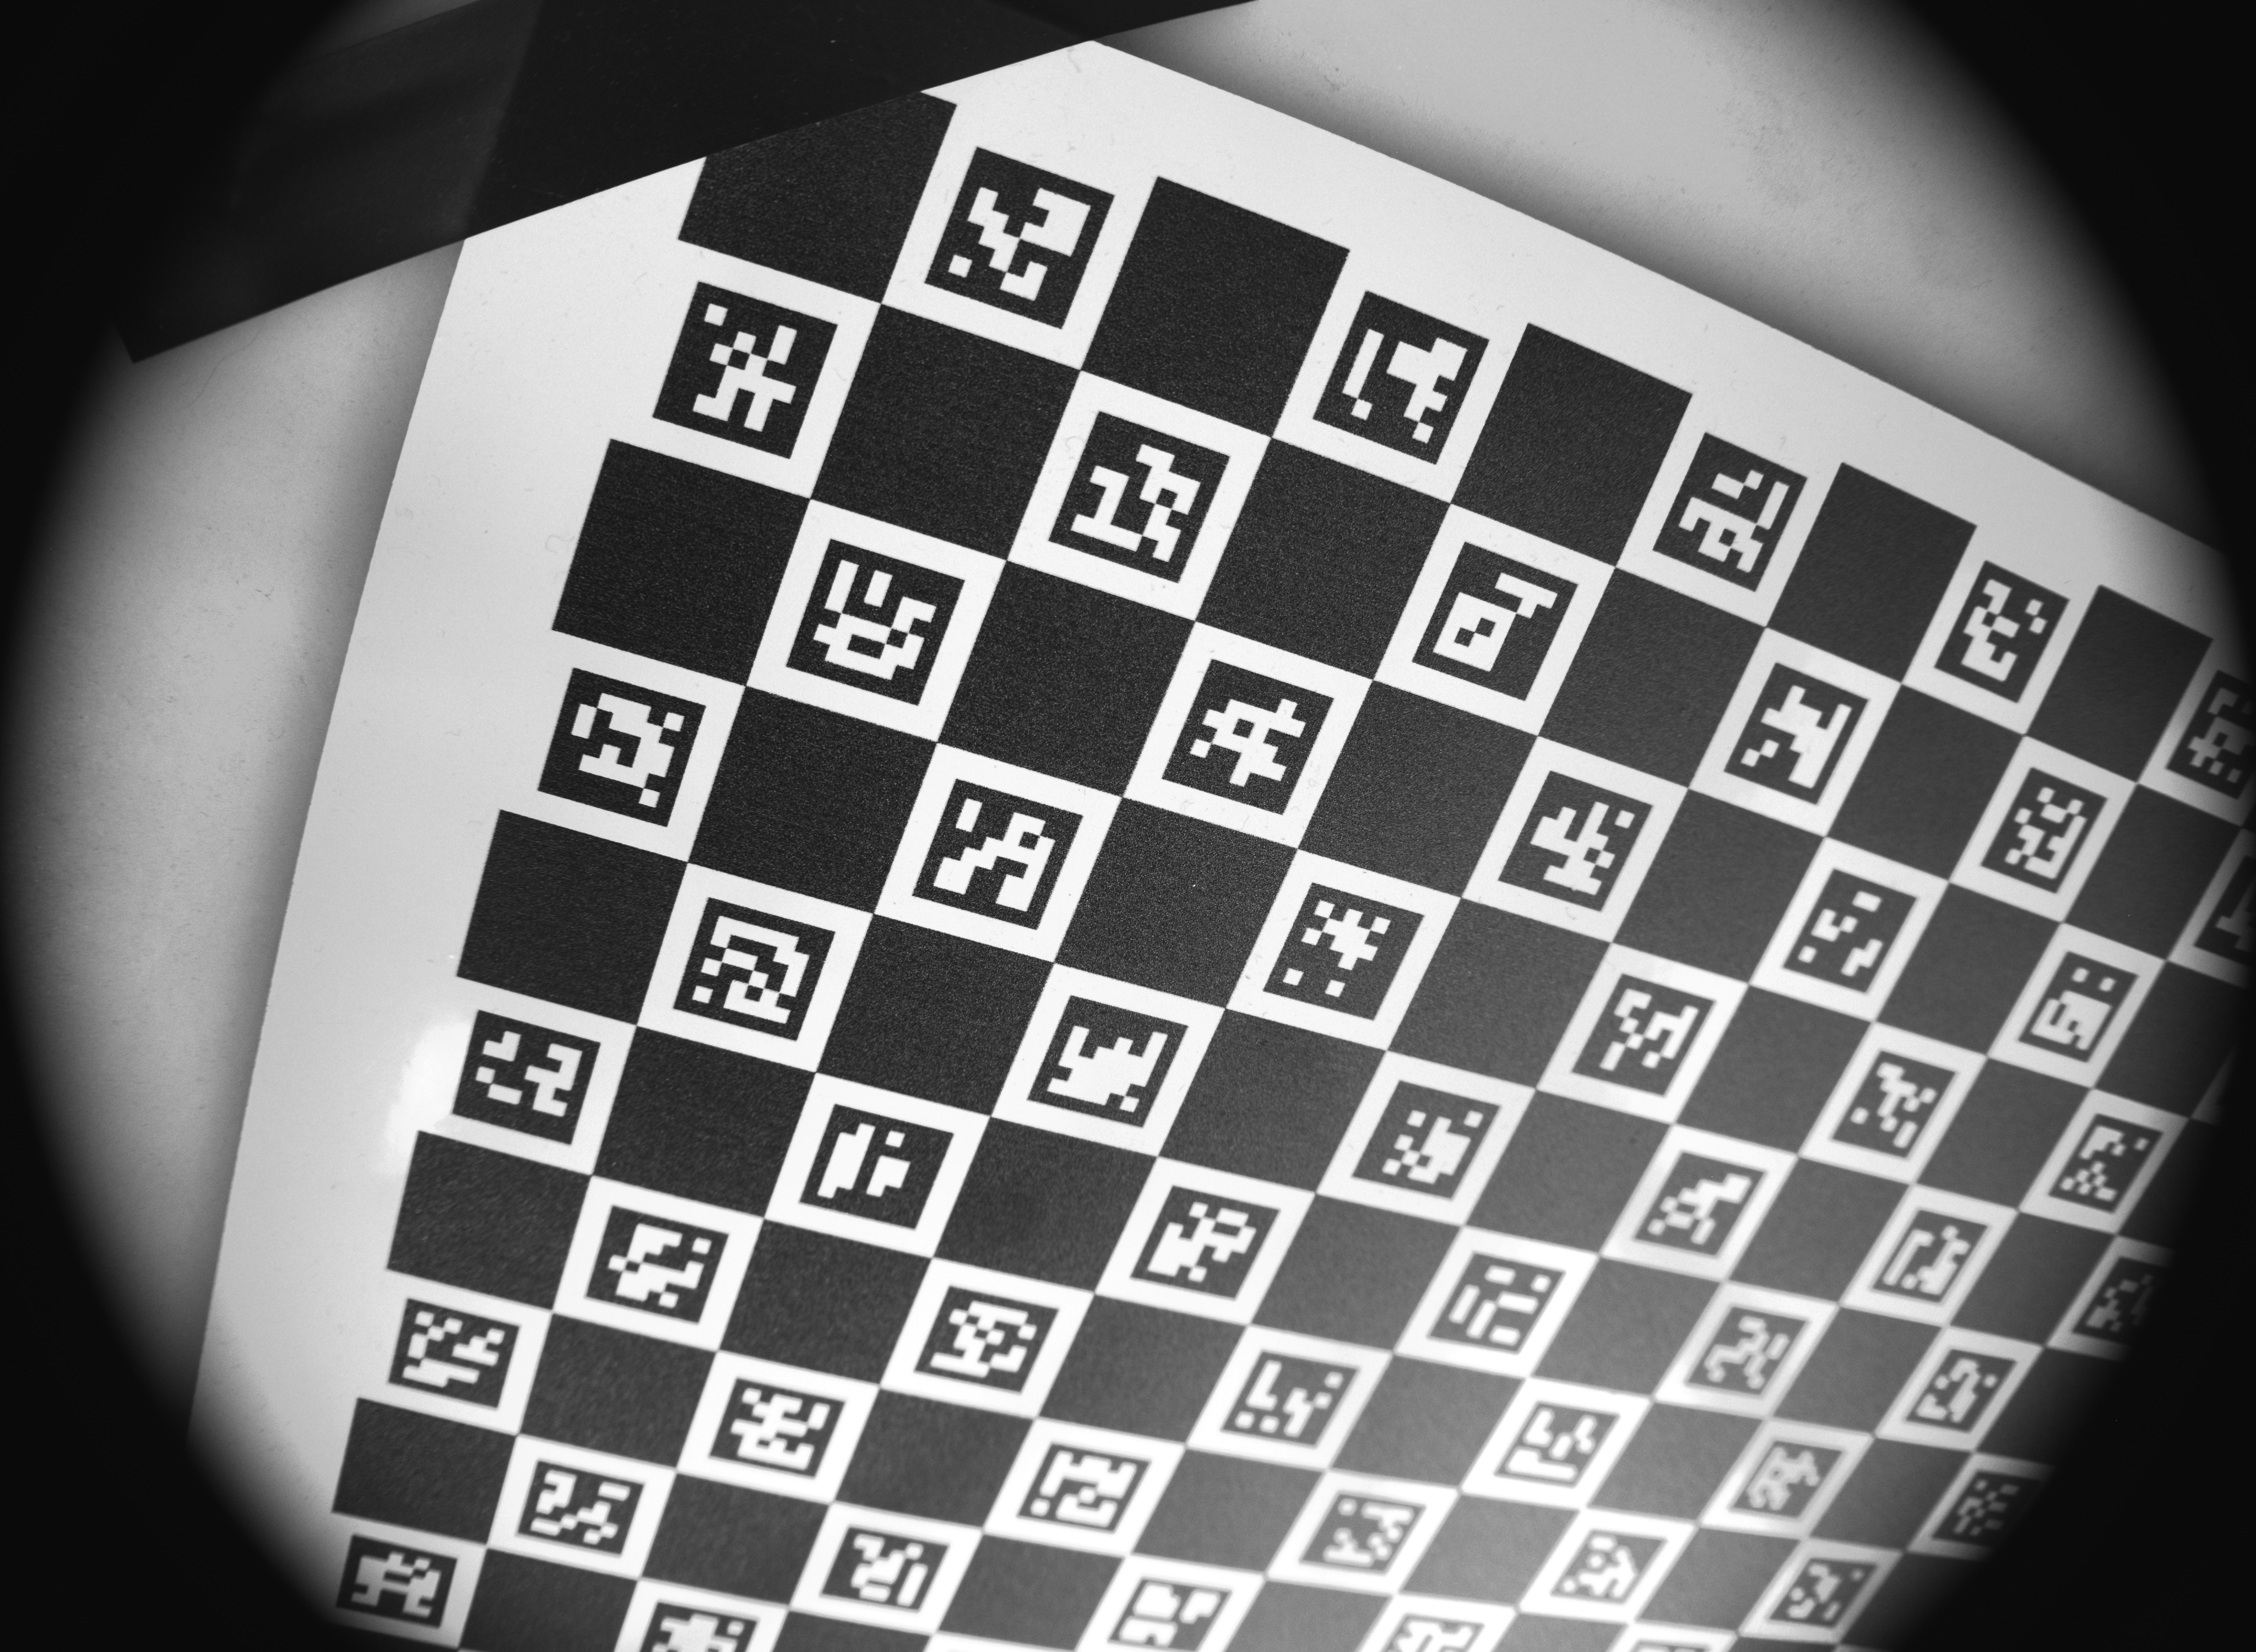
\includegraphics[width=\textwidth]{images/chapter5Images/001.png}
		\caption{Example of a high-angle or oblique observation of the target.}
		\label{fig:viewpoint_2}
	\end{subfigure}
	\hfill
	% --- Placeholder subfigure 4 ---
	\begin{subfigure}[t]{0.48\textwidth}
		\centering
		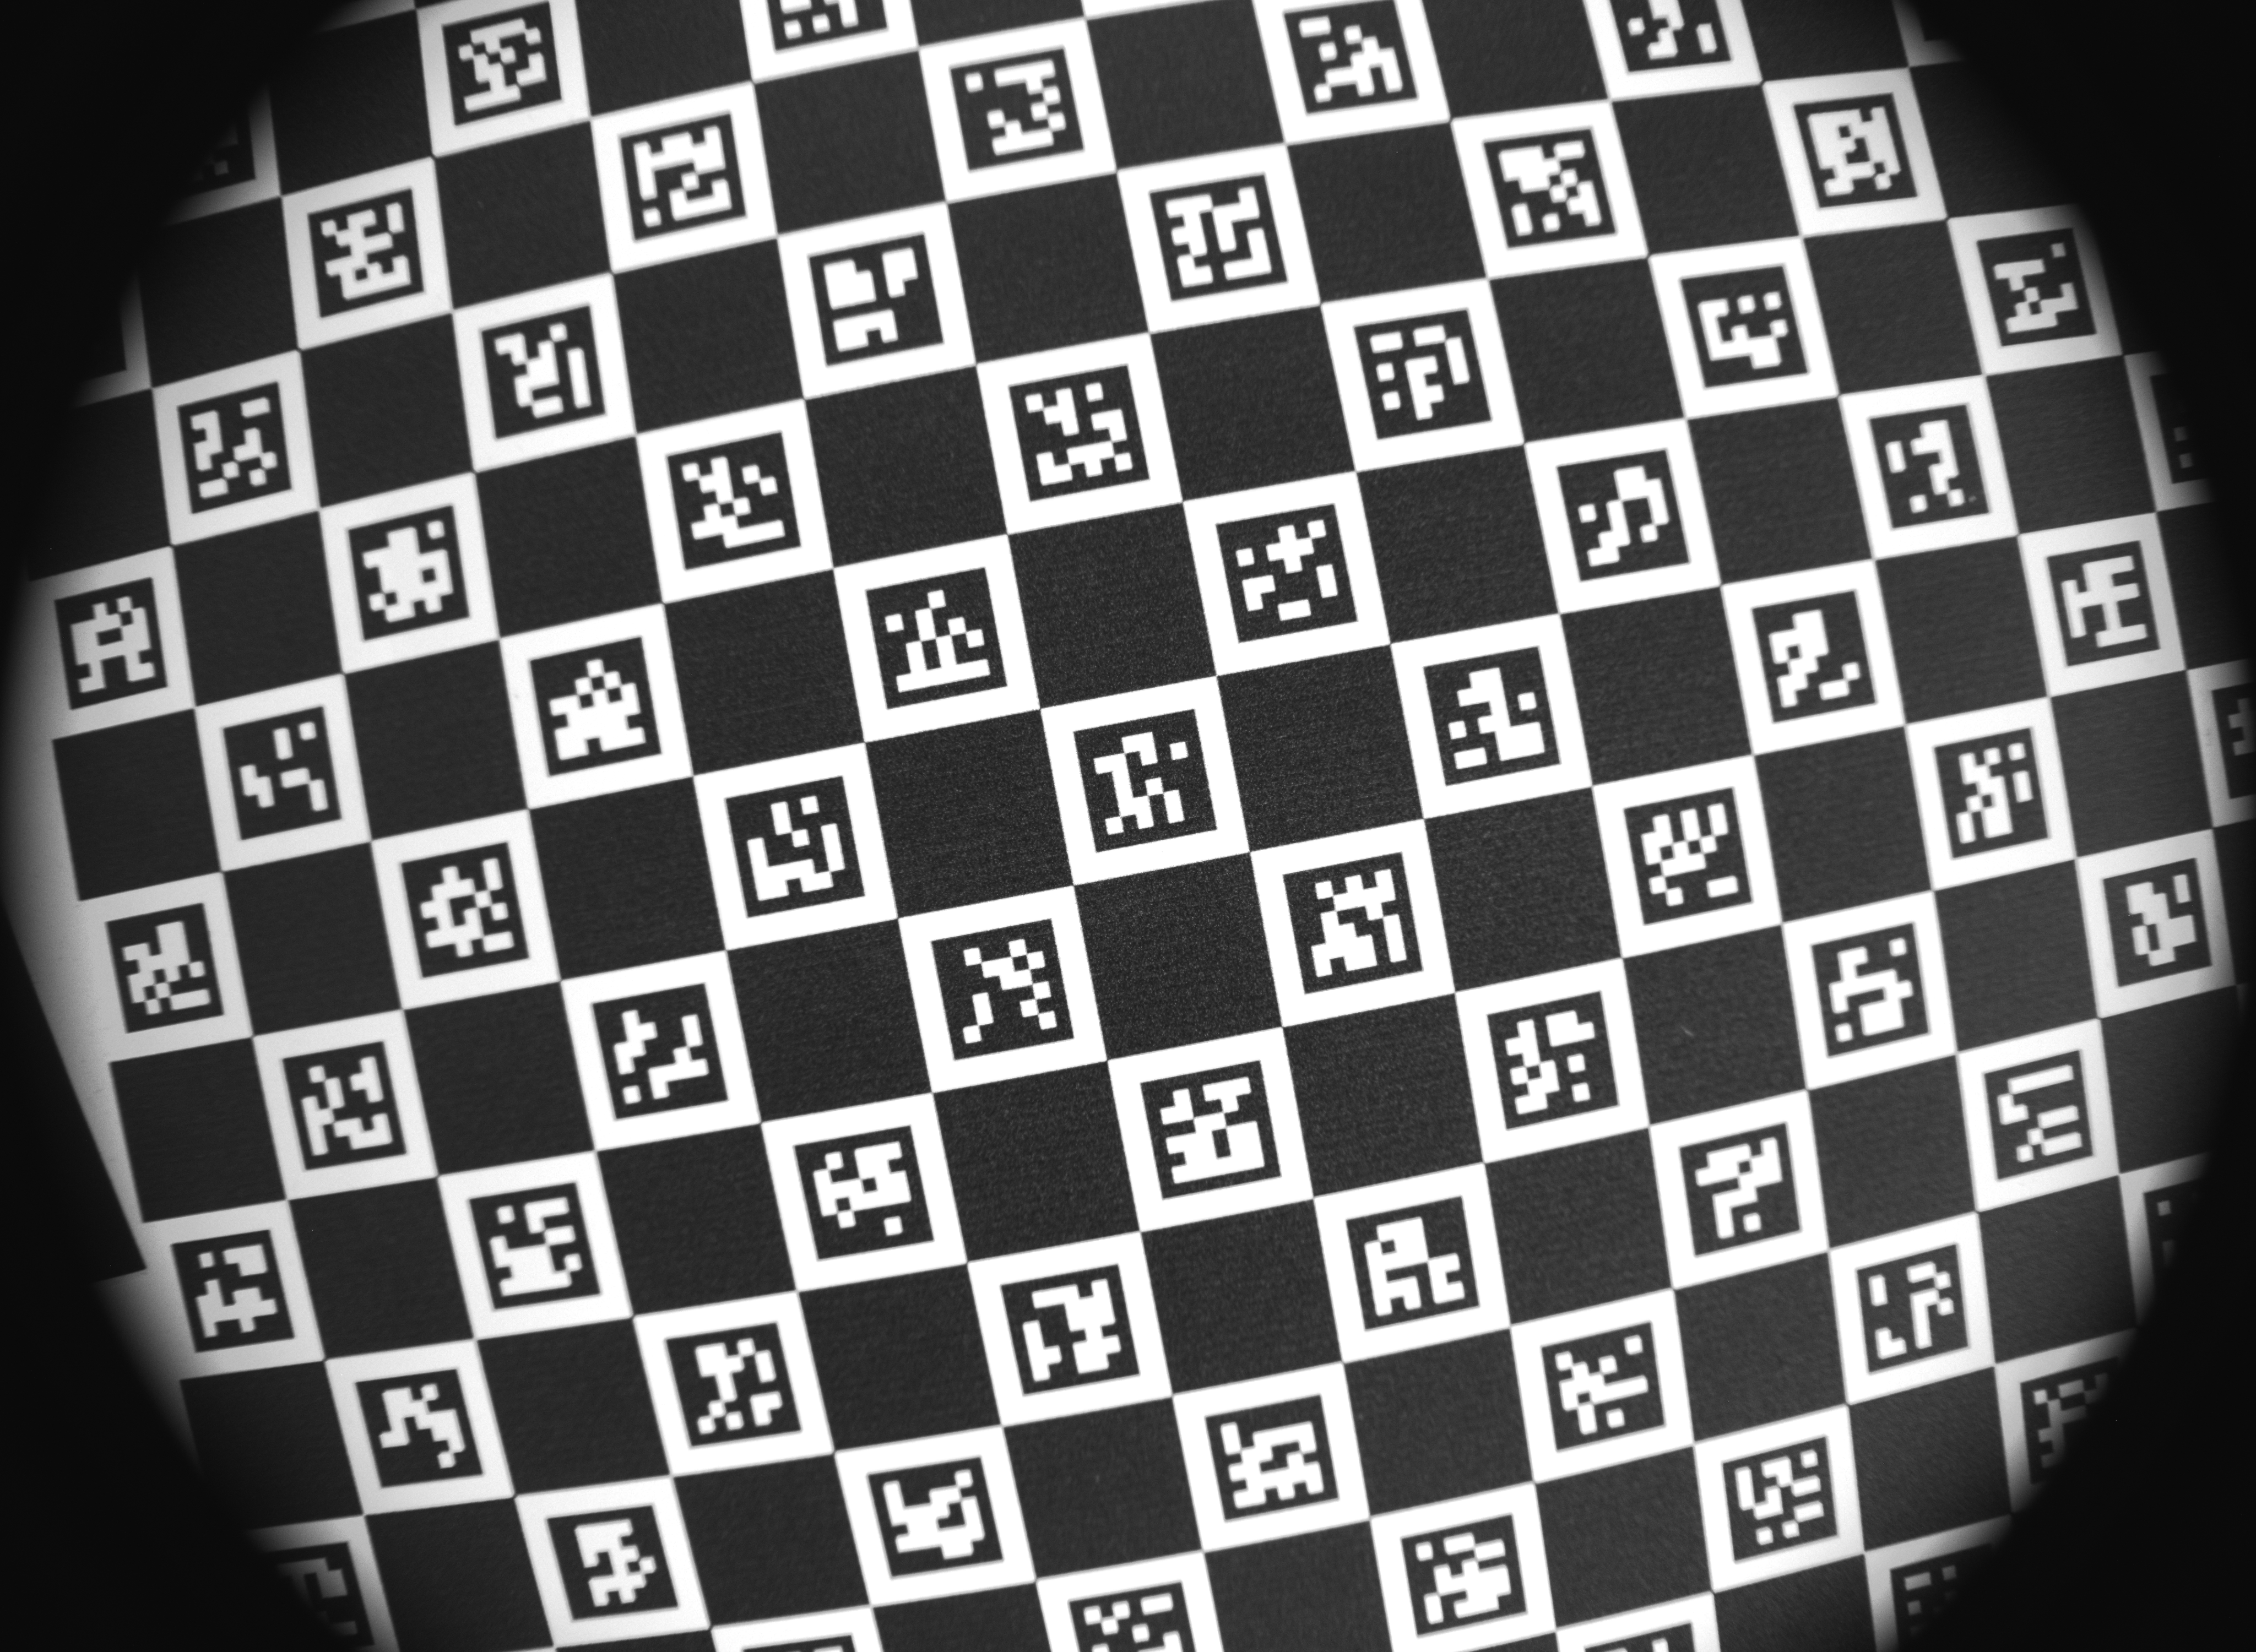
\includegraphics[width=\textwidth]{images/chapter5Images/000.png}
		\caption{Example of a a low-angle or oblique observation of the target.}
		\label{fig:viewpoint_3}
	\end{subfigure}
	
	\caption{Examples of acquired viewpoints used during dataset collection. The images highlight the variability in robot poses and camera perspectives relative to the fixed ChArUco calibration target.}
	\label{fig:dataset_viewpoints}

	
\end{figure}

\noindent This variability in viewpoints is essential to ensure that the resulting dataset satisfies the observability conditions required for stable and accurate hand-eye calibration.








\subsection{Dataset Preparation}
\label{subsec:dataset_preparation}

The datasets used throughout the experimental evaluation were generated according to the acquisition protocol described in Section~\ref{subsec:experimental_protocol}. Each observation consists of a synchronized pair composed of a robot pose ${}^B_E\mathbf{T}^{(k)}$ and a corresponding image of the ChArUco calibration target. Together, these observations form the input data required for pose estimation and subsequent hand-eye calibration.

Particular attention was devoted during acquisition to ensuring the quality of the collected observations. Since the robot was operated manually, image quality could be verified immediately after each acquisition. Observations affected by evident issues such as severe blur, inadequate target visibility, or acquisition errors were discarded and reacquired before being included in the final dataset. Consequently, the datasets used for the experiments consist exclusively of observations considered suitable for reliable feature detection and pose estimation.

\paragraph{Observation quality criteria}

For an observation to be considered valid, a number of quality requirements had to be satisfied. In particular:

\begin{itemize}
	\item the ChArUco board had to be clearly visible within the camera field of view;
	

	\item a sufficient number of ChArUco corners had to be successfully detected and identified;
	
	\item image sharpness had to allow accurate sub-pixel corner refinement;
	
	\item the estimated target pose had to exhibit a low reprojection error, indicating geometric consistency between the detected image features and the known board model.
	
	
\end{itemize}

These requirements help reduce the impact of image noise, feature localization inaccuracies, and pose estimation errors, thereby improving the reliability of the calibration results.



\paragraph{Examples of valid and invalid observations}

Figure~\ref{fig:dataset_examples} presents representative examples of images acquired during the data collection process. Figure~\ref{fig:valid_observation} shows a valid observation in which the ChArUco board is fully visible and a large number of corners are successfully detected. Figures~\ref{fig:blurred_observation} and~\ref{fig:cropped_observation} illustrate examples of acquisition conditions that may compromise calibration quality, namely image blur and insufficient target visibility.

Although such observations were not included in the final datasets, they are presented here to illustrate the practical considerations involved in collecting high-quality calibration data.

\begin{figure}[htbp]
	\centering
	

	% ------------------------------------------------
	% Valid image
	% ------------------------------------------------
	\begin{subfigure}[t]{0.32\textwidth}
		\centering
		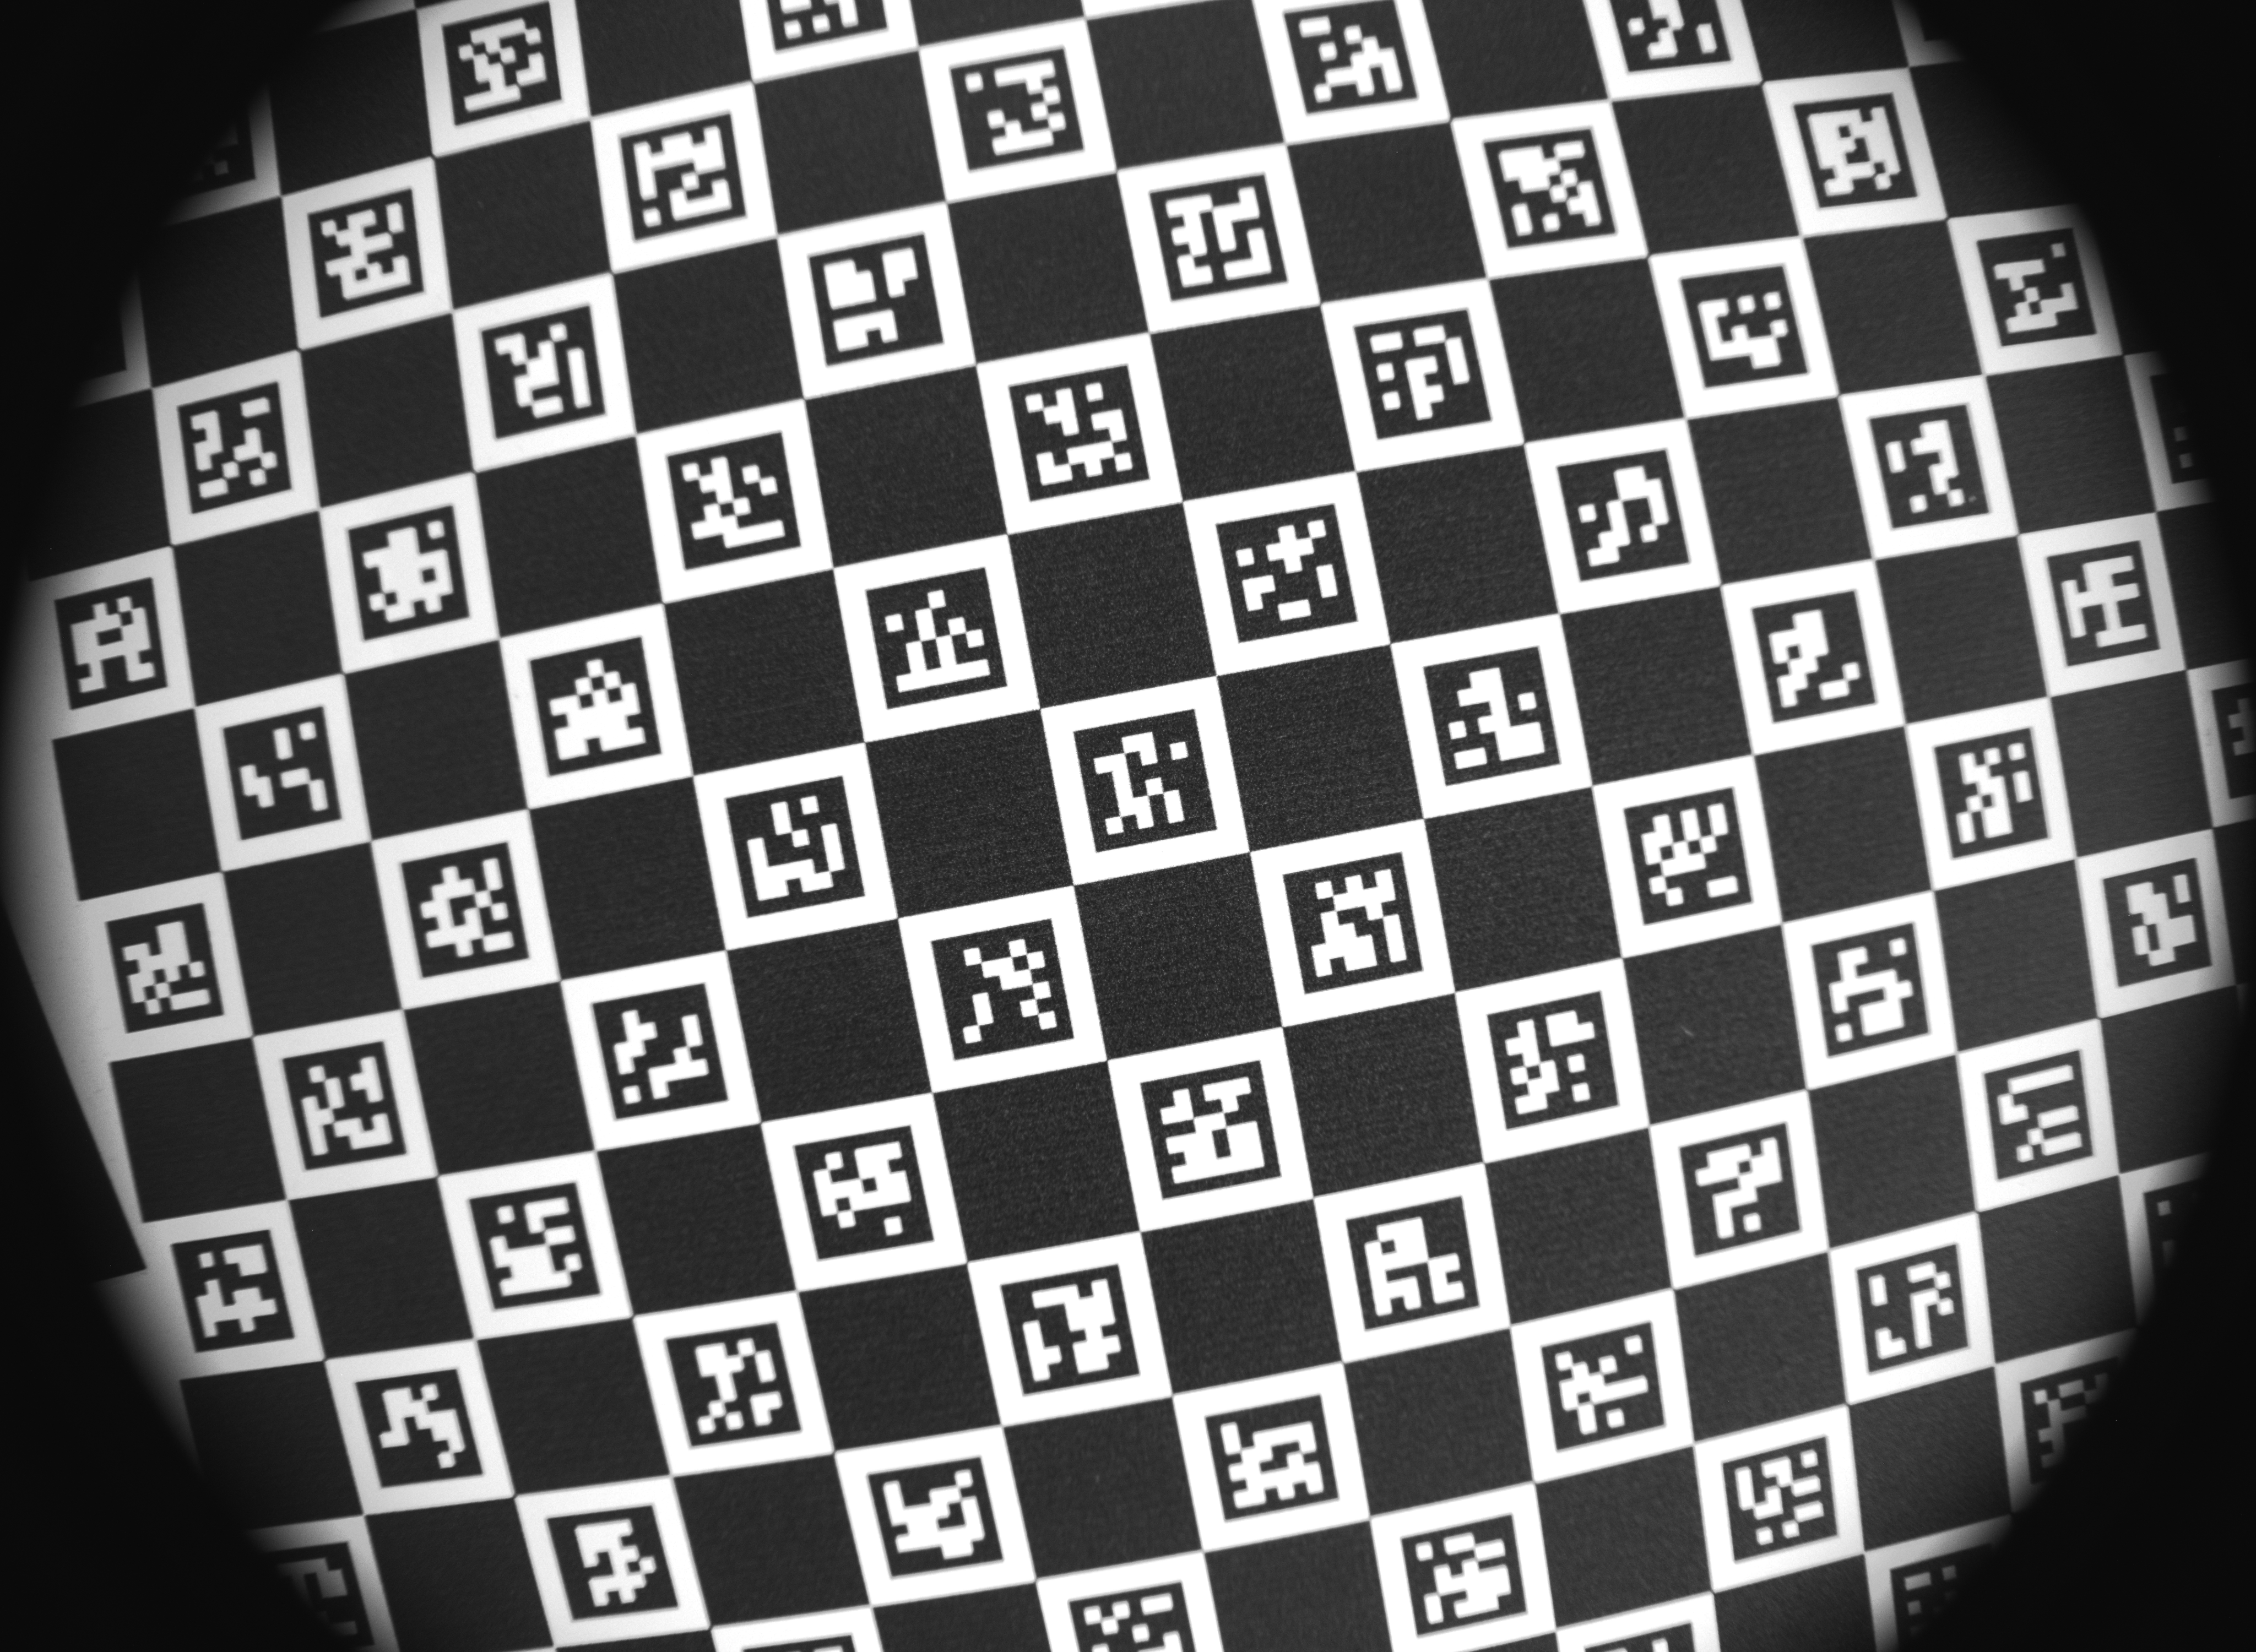
\includegraphics[width=\textwidth]{images/chapter5Images/000.png}
		\caption{Valid observation with detected ChArUco corners.}
		\label{fig:valid_observation}
	\end{subfigure}
	\hfill
	
	% ------------------------------------------------
	% Blurred image
	% ------------------------------------------------
	\begin{subfigure}[t]{0.32\textwidth}
		\centering
		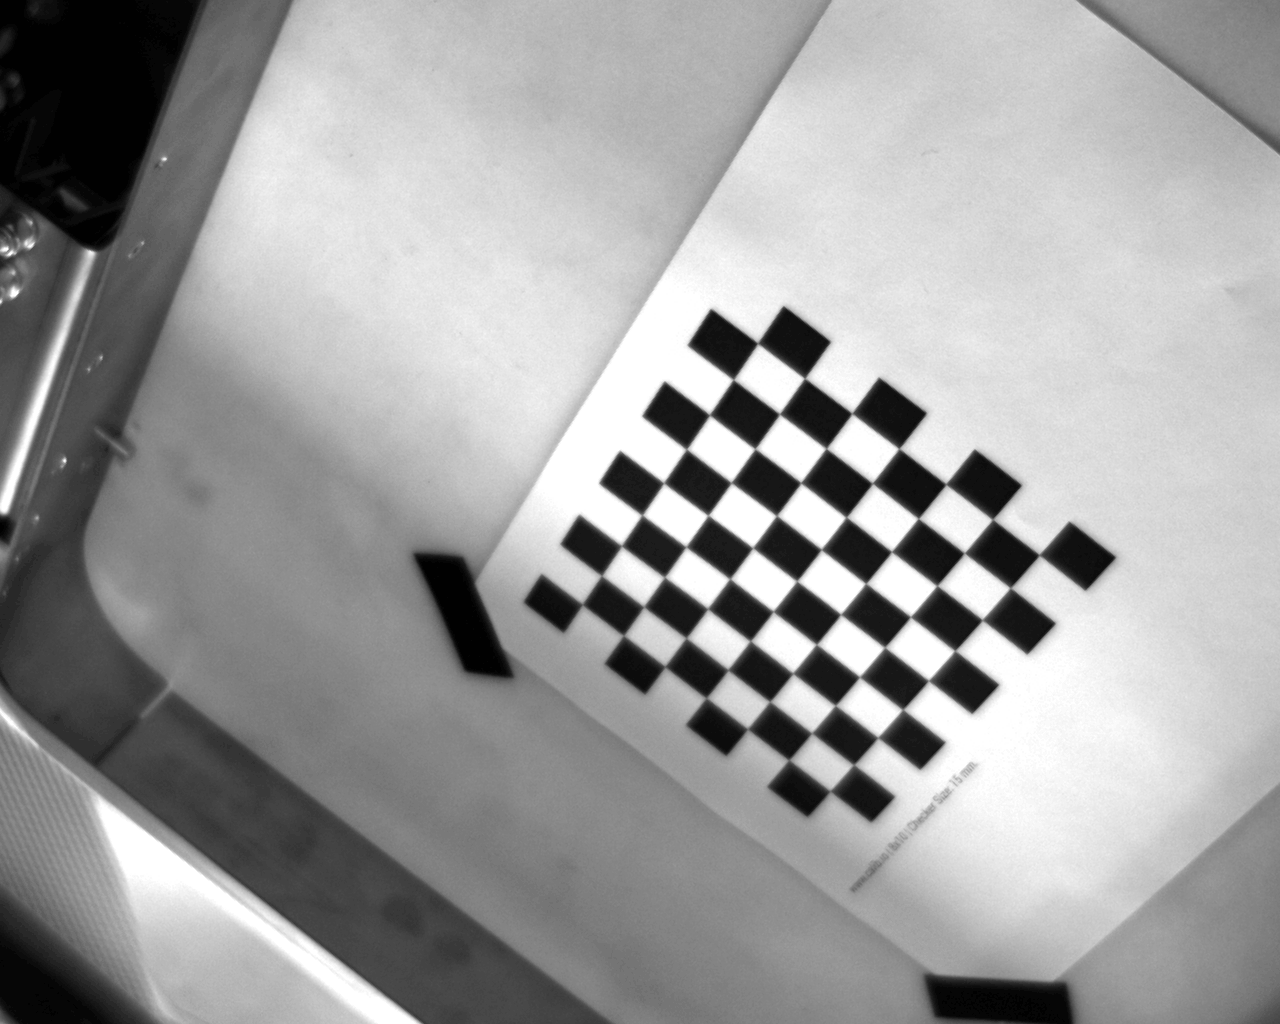
\includegraphics[width=\textwidth]{images/chapter5Images/motion_blur.png}
		\caption{Image affected by blur.}
		\label{fig:blurred_observation}
	\end{subfigure}
	\hfill
	
	% ------------------------------------------------
	% Cropped board
	% ------------------------------------------------
	\begin{subfigure}[t]{0.32\textwidth}
		\centering
		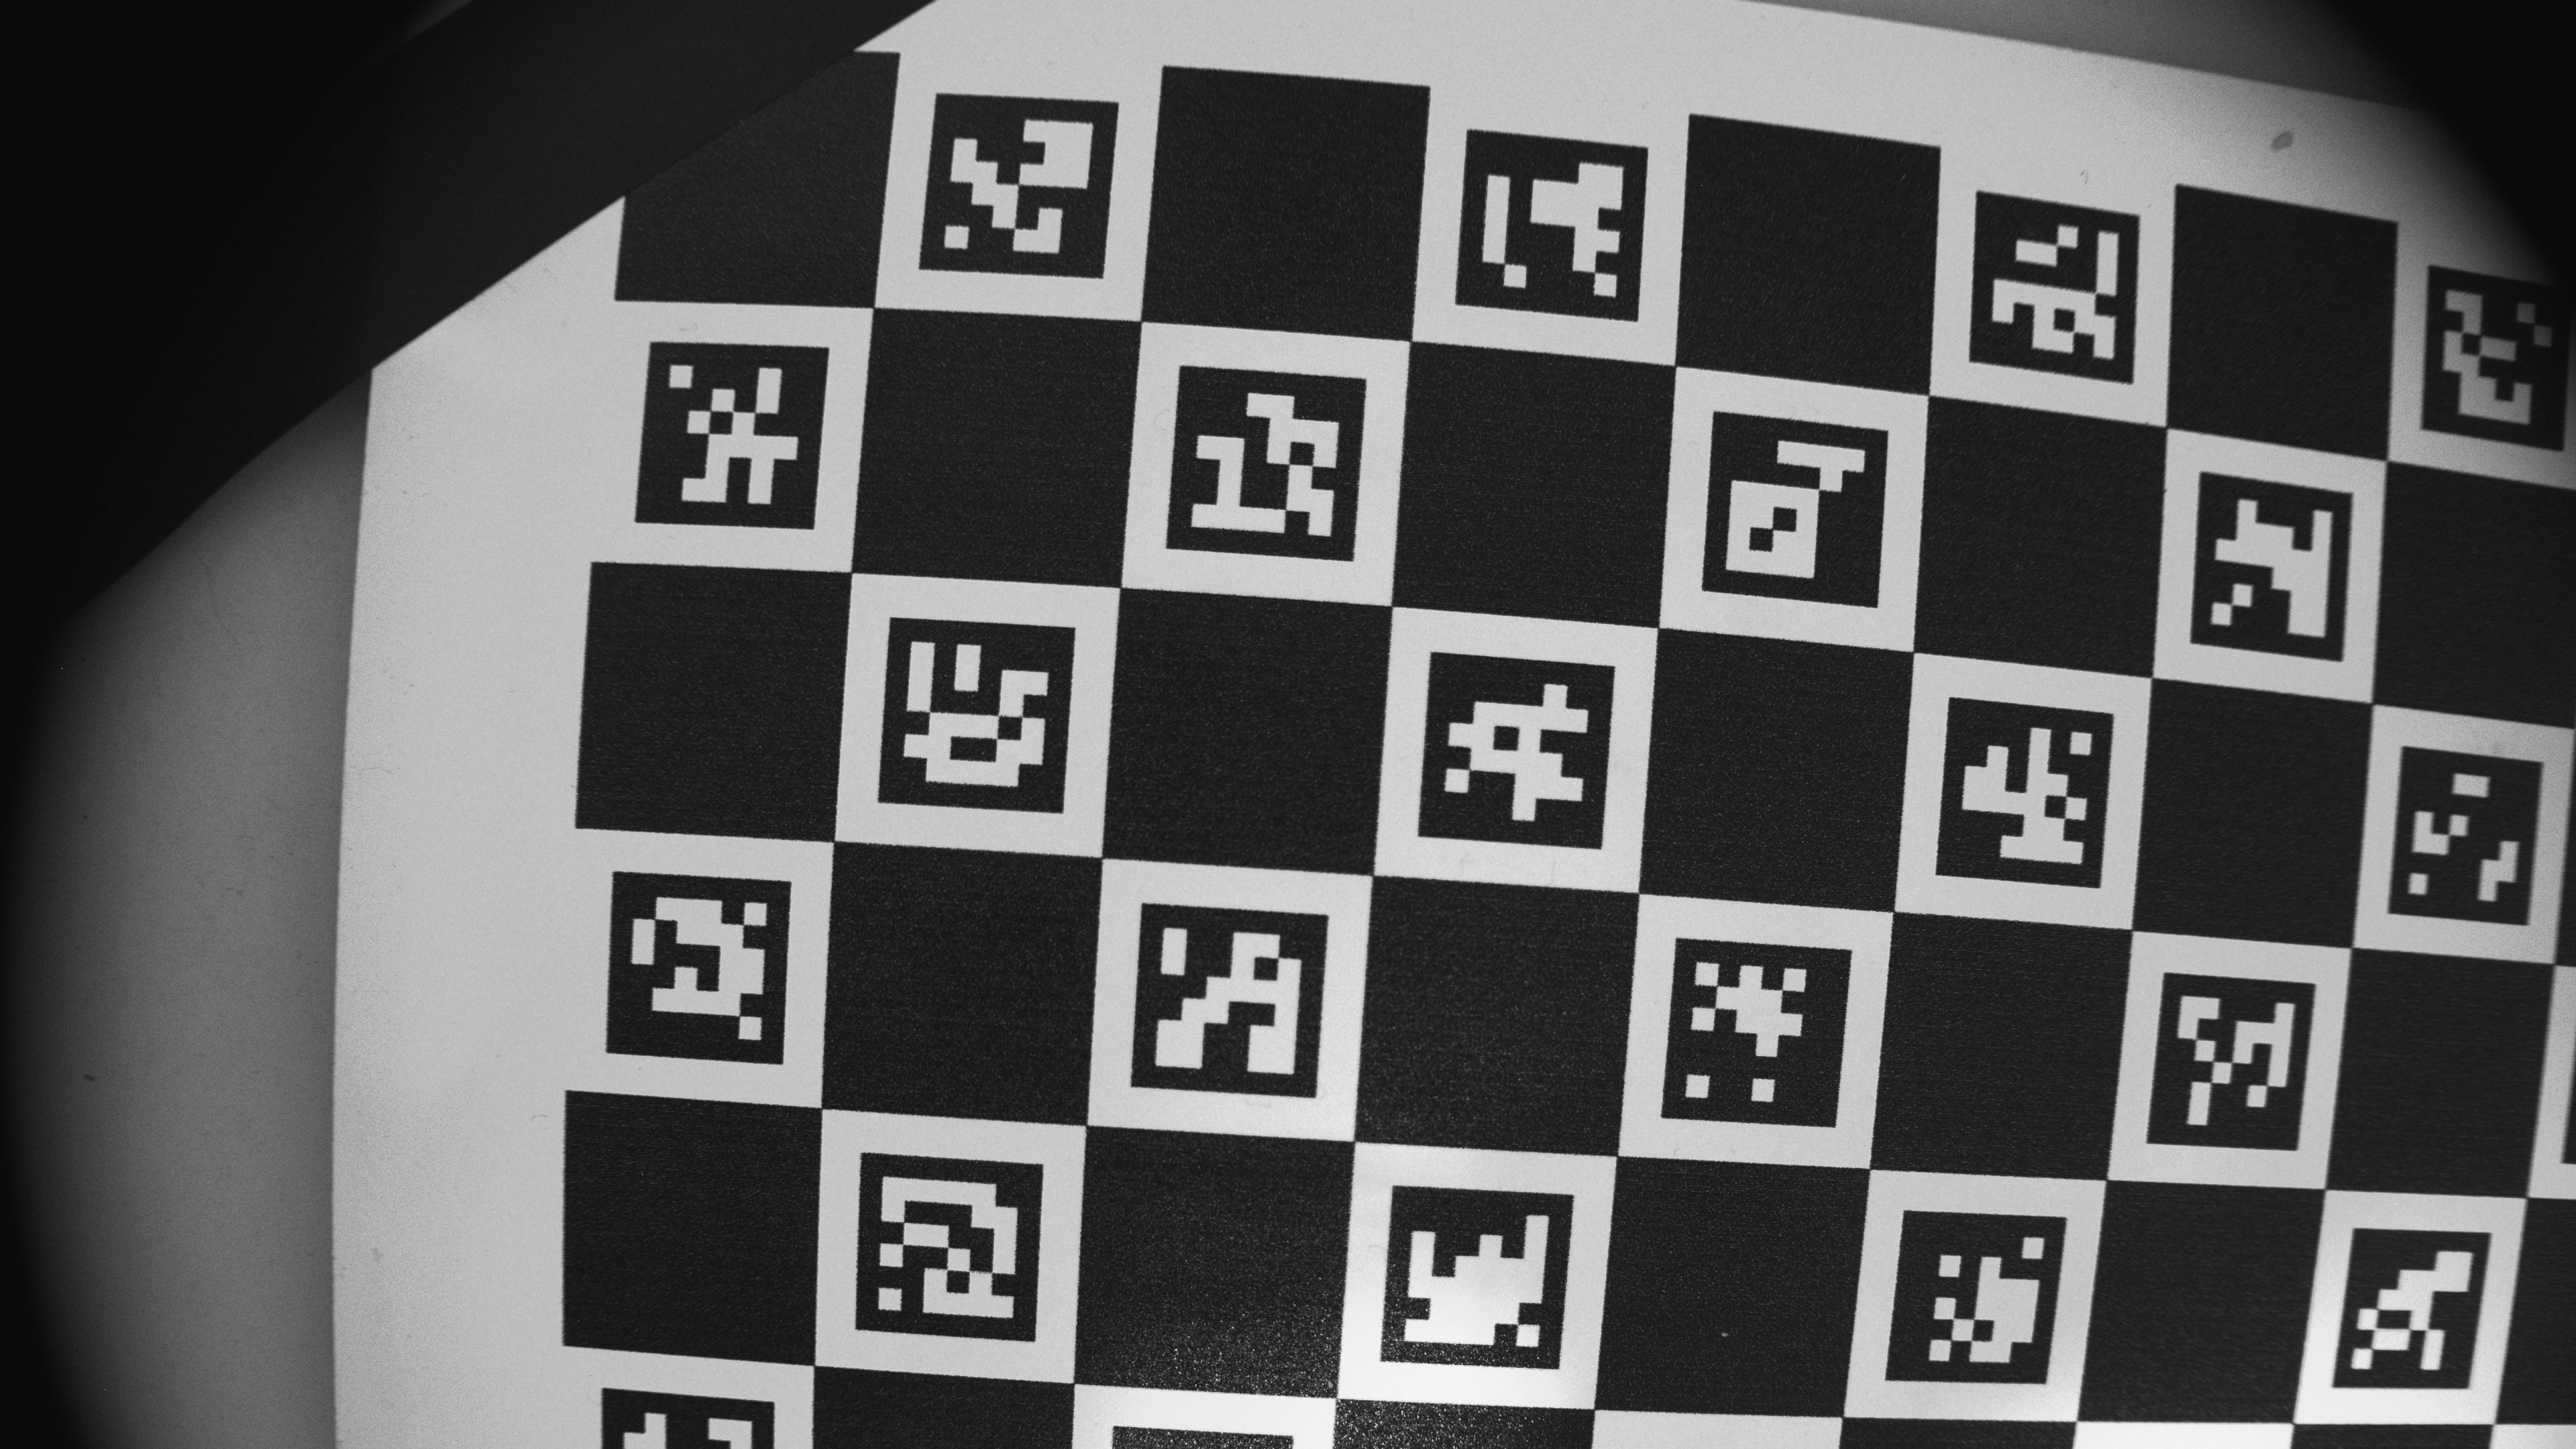
\includegraphics[width=\textwidth]{images/chapter5Images/insufficient_corners.png}
		\caption{Insufficient target visibility.}
		\label{fig:cropped_observation}
	\end{subfigure}
	
	\caption{Representative examples of observations acquired during the experimental campaign. Only observations satisfying the quality criteria described in this section were included in the final calibration datasets.}
	\label{fig:dataset_examples}

	
\end{figure}

The preparation of high-quality datasets is a critical aspect of hand-eye calibration, as errors introduced during image acquisition and feature detection directly propagate to the estimated target poses and, consequently, to the final calibration parameters. For this reason, careful attention was devoted to ensuring sufficient viewpoint diversity, reliable corner detection, and consistent observation quality throughout the acquisition process.






\subsection{Evaluation Metrics}
\label{subsec:evaluation_metrics}

The performance of the calibration pipeline was evaluated through a set of quantitative metrics designed to assess both the intrinsic camera calibration and the hand-eye calibration stages. Since the objectives of these two procedures differ, separate evaluation criteria were adopted.

\paragraph{Intrinsic calibration}

The quality of the intrinsic camera calibration was assessed using the mean reprojection error. This metric measures the discrepancy between the observed image coordinates of the detected ChArUco corners and the coordinates predicted by the calibrated camera model.

Given a set of detected image points $\tilde{\mathbf{p}}_i$ and their corresponding reprojected locations $\hat{\mathbf{p}}_i$, the reprojection error is defined as

\begin{equation}
	e_{\mathrm{repr}} =
	\frac{1}{N}
	\sum_{i=1}^{N}
	\left|
	\tilde{\mathbf{p}}_i -
	\hat{\mathbf{p}}_i
	\right|_2 ,
	\label{eq:mean_reprojection_error}
\end{equation}

where $N$ denotes the total number of observed corners. The resulting value is expressed in pixels and provides an indication of how accurately the calibrated camera model explains the observed image measurements.

Lower reprojection errors generally indicate a more accurate estimation of the camera intrinsic parameters and lens distortion coefficients.

\paragraph{Hand-eye calibration}

Unlike intrinsic calibration, the quality of a hand-eye calibration cannot be directly assessed through image reprojection alone. A calibration may yield a low reprojection error while still producing inconsistent spatial reconstructions when observations from multiple viewpoints are combined.

For this reason, the primary evaluation metric adopted in this work is a \textit{cross-image consistency} measure based on the reconstructed three-dimensional positions of the ChArUco corners.

For each detected corner, its position is independently reconstructed in the robot base frame using every image in which that corner is visible. Ideally, all reconstructed positions associated with the same physical corner should coincide. In practice, calibration inaccuracies, pose estimation errors, and image noise introduce small discrepancies between these estimates.

Let

\begin{equation}
	\mathbf{p}_1,\mathbf{p}_2,\ldots,\mathbf{p}_M
\end{equation}

be the reconstructed positions of a given corner expressed in the robot base frame. The centroid of these observations is computed as

\begin{equation}
	\mathbf{c}
	=
	\frac{1}{M}
	\sum_{i=1}^{M}
	\mathbf{p}_i
	\label{eq:centroid}
\end{equation}

The consistency of the reconstruction is then quantified through the mean Euclidean distance of the reconstructed points from their centroid:

\begin{equation}
	e_{\mathrm{cons}}
	=
	\frac{1}{M}
	\sum_{i=1}^{M}
	\left\|
	\mathbf{p}_i-\mathbf{c}
	\right\|_2
	\label{eq:consistency_metric}
\end{equation}






This metric provides a direct measure of the spatial dispersion of the reconstructed corner positions. Smaller values indicate that the reconstructed points are tightly clustered and therefore that the estimated hand-eye transformation is geometrically consistent across multiple observations.

The consistency metric was computed for every ChArUco corner observed in at least two images. Global calibration performance was then evaluated by averaging the consistency values across all valid corners.

To provide a visual interpretation of the metric, Figure~\ref{fig:reprojection_examples} shows representative reprojection results obtained after calibration. For clarity, a standard chessboard pattern is used instead of a ChArUco board, since the corner locations are easier to visualize. In each image, the green markers indicate the detected corner positions extracted from the image, while the red markers represent the corresponding corner positions obtained by reprojection using the estimated camera pose and calibration parameters.

When the calibration is accurate, the detected and reprojected corners overlap almost perfectly, resulting in sub-pixel discrepancies that are barely visible. Conversely, larger calibration errors manifest as a systematic separation between the two sets of points. The example shown in Figure~\ref{fig:reprojection_examples}(c) illustrates a case where a residual board tilt introduces a noticeable reprojection error of approximately 1.5 mm, producing a visible displacement between the detected and reprojected corner locations.


\begin{figure}[htbp]
	\centering
	
	\begin{subfigure}[t]{0.32\textwidth}
		\centering
		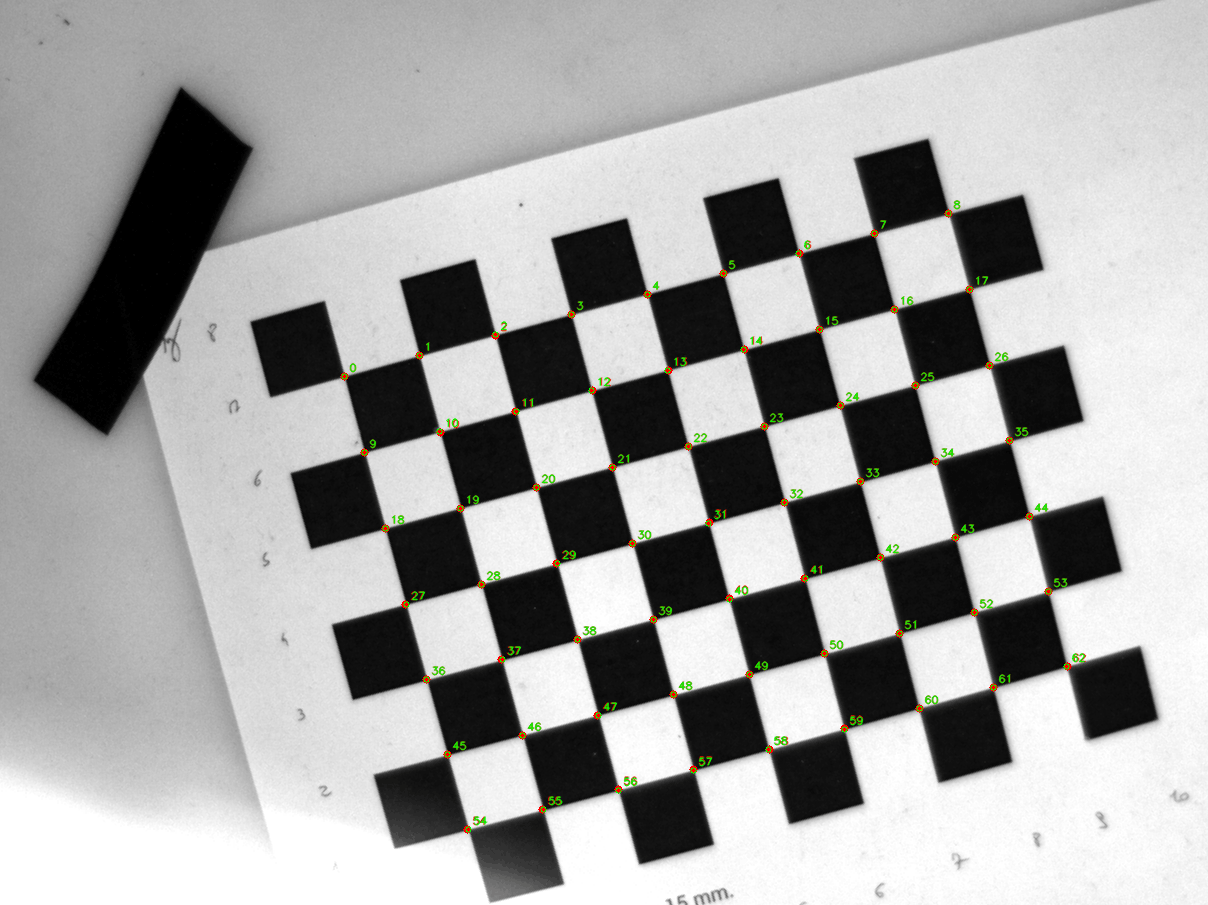
\includegraphics[width=\textwidth]{images/chapter5Images/reprojection.png}
		\caption{Accurate calibration.}
	\end{subfigure}
	
	\begin{subfigure}[t]{0.32\textwidth}
		\centering
		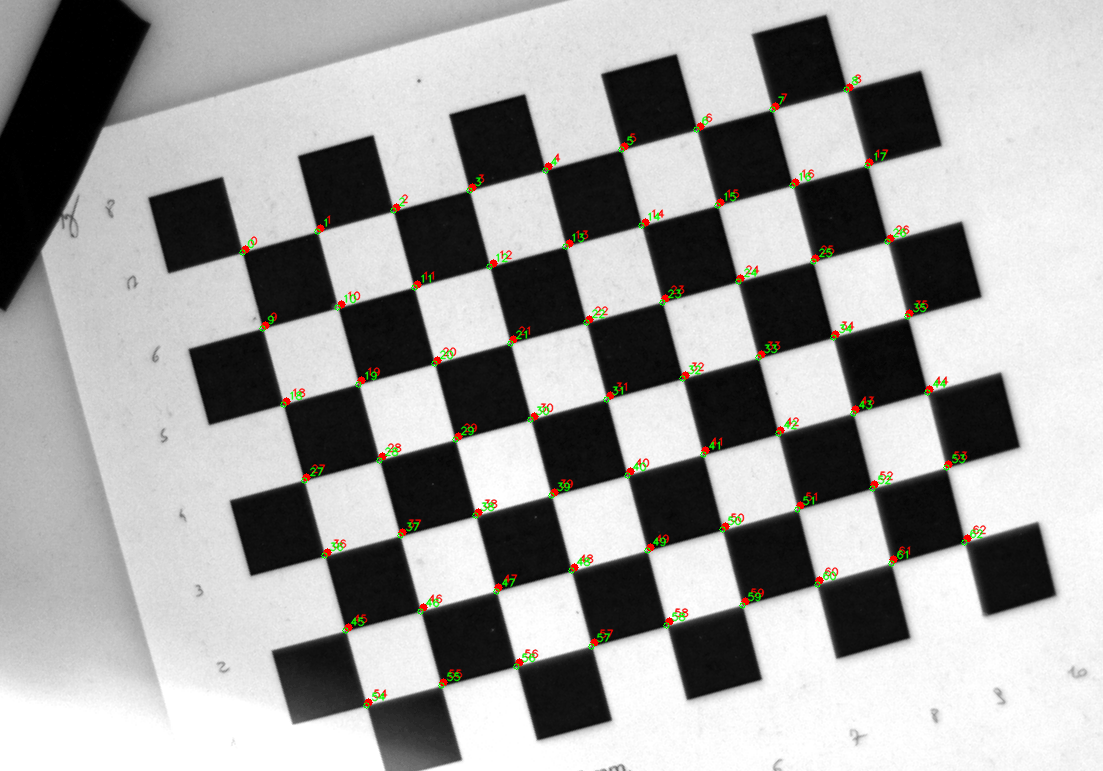
\includegraphics[width=\textwidth]{images/chapter5Images/reprojection_bad.png}
		\caption{Residual board tilt producing approximately 1.5 mm error.}
	\end{subfigure}
	
	\caption{Examples of reprojection results after calibration. Green markers correspond to detected chessboard corners, while red markers indicate the reprojected corner positions obtained from the estimated camera pose and calibration parameters. The first example show near-perfect alignment, whereas the second example highlights the effect of residual board tilt on reprojection accuracy.}
	\label{fig:reprojection_examples}
\end{figure}


The combination of reprojection error and cross-image consistency enables both image-space accuracy and spatial reconstruction accuracy to be evaluated, providing a comprehensive assessment of the overall calibration quality.



\section{Calibration Results}



\subsection{Intrinsic Calibration Results}
\label{subsec:intrinsic_results}

During the preliminary stages of the experimental campaign, intrinsic calibration was initially performed using a Cognex CAM-CIC-1300-60GC industrial camera. Although the camera provided reliable image acquisition capabilities, its resolution of 1280 × 1024 pixels limited the spatial accuracy of ChArUco corner localization, particularly when the calibration target occupied only a portion of the image.

To improve measurement precision, the camera was subsequently replaced with a Cognex CAM-CIC-12-9C-IP67 industrial camera equipped with a 12 MP sensor (4096 × 3000 pixels). The significantly higher image resolution increased the number of pixels covering each ChArUco corner, enabling more accurate sub-pixel localization and more stable pose estimation results.

For this reason, all hand-eye calibration experiments presented in the remainder of this chapter were conducted using the 12 MP camera. The preliminary results obtained with the CAM-CIC-1300-60GC are nevertheless reported for comparison purposes.

The camera system used in this work was intentionally selected to operate under challenging optical conditions. In particular, a lens exhibiting strong radial distortion (comparable to a wide-angle or fisheye-like configuration) was employed. This choice was motivated by the desire to stress-test the intrinsic calibration pipeline under non-ideal imaging conditions and to verify the robustness of the distortion model beyond standard industrial setups.

Table~\ref{tab:intrinsic_comparison} summarizes the intrinsic calibration results obtained for the two cameras.

\begin{table}[htbp]
	\centering
	\caption{Comparison of intrinsic calibration results obtained using the evaluated cameras.}
	\label{tab:intrinsic_comparison}
	\begin{tabular}{lccc}
		\toprule
		Camera & Resolution & Images & Reprojection Error (px) \\
		\midrule
		Cognex CAM-CIC-1300-60GC & 1280 $\times$ 1024 & 20 & 1.24 \\
		Cognex CAM-CIC-12-9C-IP67 & 4096 $\times$ 3000 & 20 & 0.68 \\
		\bottomrule
	\end{tabular}
\end{table}
The higher-resolution Cognex camera achieved a lower reprojection error and provided significantly more accurate corner localization. In addition, the increased sensor resolution enabled the ChArUco board corners to be detected with greater spatial precision, resulting in more stable pose estimates across different viewpoints. For these reasons, all subsequent hand-eye calibration experiments were performed using the Cognex camera.


Figure~\ref{fig:intrinsic_undistortion} illustrates the effect of image undistortion using the estimated intrinsic parameters and distortion coefficients. Despite the presence of strong radial distortion, which produces visible geometric deformation near the image boundaries, the calibration model is able to recover a geometrically consistent rectified image. In the original images, straight structures appear significantly curved, with deviations reaching the order of centimetres at the image periphery when mapped onto the calibration plane. After undistortion, these structures are restored to near-linear geometry, confirming the validity of the estimated distortion model.

\begin{figure}[htbp]
	\centering
	

	\begin{subfigure}[t]{0.48\textwidth}
		\centering
		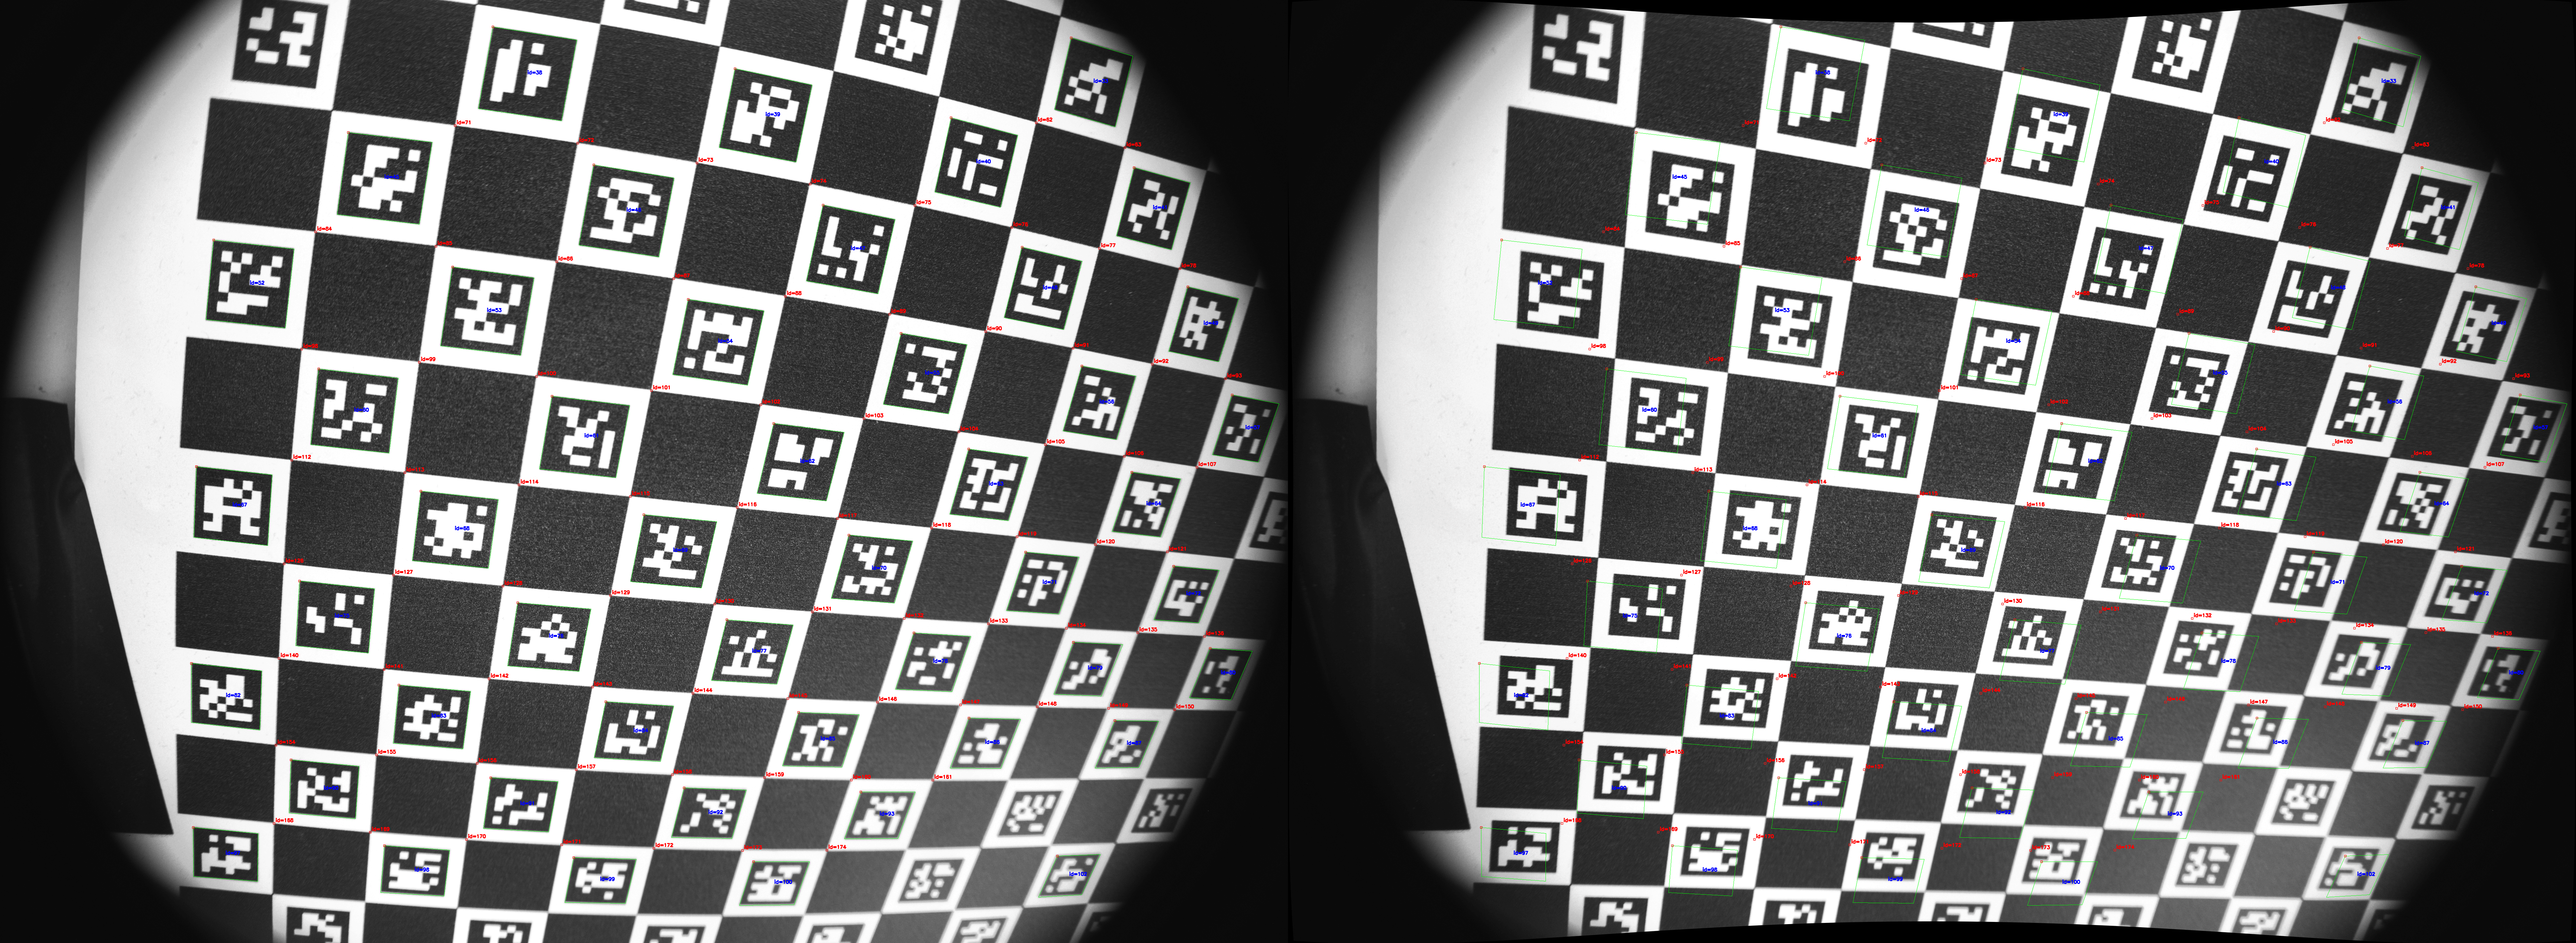
\includegraphics[width=\textwidth]{images/chapter2Images/005_comparison_markers.png}
		\caption{Original image and undistorted image.}
		\label{fig:original_image}
	\end{subfigure}
	
	
	\caption{Example of image correction obtained using the estimated intrinsic parameters and distortion coefficients.}
	\label{fig:intrinsic_undistortion}

	
\end{figure}

The final intrinsic parameters obtained for the Cognex camera are reported in Table~\ref{tab:intrinsic_parameters}. For completeness, the corresponding intrinsic matrix is reported in Equation~\eqref{eq:final_intrinsic_matrix}.

\begin{table}[htbp]
	\centering
	\caption{Estimated intrinsic parameters of the Cognex camera.}
	\label{tab:intrinsic_parameters}
	\begin{tabular}{lc}
		\toprule
		Parameter & Value \\
		\midrule
		$f_x$ & 2448.22 px \\
		$f_y$ & 2456.20 px \\
		$c_x$ & 656.23 px \\
		$c_y$ & 526.47 px \\
		$k_1$ & -0.2332 \\
		$k_2$ & -220.7575 \\
		$p_1$ & 0.000911 \\
		$p_2$ & 0.001356 \\
		$k_3$ & -79.3936 \\
		\bottomrule
	\end{tabular}
\end{table}

\begin{equation}
	\mathbf{K}
	=
	\begin{bmatrix}
		f_x & 0 & c_x \\
		0 & f_y & c_y \\
		0 & 0 & 1
	\end{bmatrix}
	=
	\begin{bmatrix}
		2448.215 & 0 & 656.232 \\
		0 & 2456.203 & 526.467 \\
		0 & 0 & 1
	\end{bmatrix}
	\label{eq:final_intrinsic_matrix}
\end{equation}

Overall, the intrinsic calibration achieved sub-pixel reprojection accuracy, indicating that the estimated camera model provides a sufficiently accurate representation of the imaging system for the purposes of pose estimation and hand-eye calibration. The resulting intrinsic parameters were therefore used throughout all subsequent experiments presented in this chapter.







\subsection{Hand-Eye Calibration Convergence}
\label{subsec}

The accuracy of hand-eye calibration depends not only on the selected calibration algorithm but also on the quantity and diversity of the acquired observations. Although a valid solution can theoretically be obtained from a relatively small number of motion pairs, practical calibration accuracy generally improves as additional observations are incorporated into the estimation process.

To investigate the influence of dataset size on calibration quality, a convergence analysis was performed using progressively larger subsets of the acquired dataset. Starting from a small number of observations, additional image--pose pairs were incrementally included and the hand-eye calibration was recomputed at each step. The resulting calibration was then evaluated using the cross-image consistency metric introduced in Section~\ref{subsec}.

\subsubsection{Consistency Error Convergence}

The first analysis evaluates the evolution of the consistency metric as a function of the number of observations used during calibration.

\begin{figure}[htbp]
	\centering
	\fbox{
		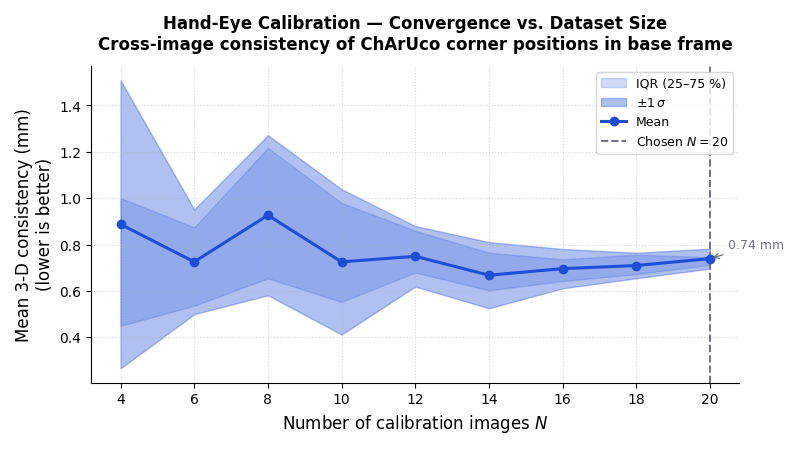
\includegraphics[width=\textwidth]{images/chapter5Images/convergence.png}
	}
	\caption{Evolution of the cross-image consistency error as a function of dataset size.}
	\label{fig:consistency_convergence}
	
\end{figure}

Figure~\ref{fig} shows that the consistency error decreases as additional observations are incorporated into the calibration process. For small datasets, the estimated hand-eye transformation exhibits greater variability, resulting in larger spatial discrepancies between independent reconstructions of the same ChArUco corners.

As the number of observations increases, the consistency error progressively decreases, indicating improved agreement among the reconstructed corner positions. This behaviour is expected, since larger datasets provide a richer set of geometric constraints and reduce the influence of individual measurement errors.

Beyond approximately \textit{15} observations, the consistency error reaches a near-stable value and further improvements become marginal. This suggests that the calibration process has effectively converged and that additional observations provide diminishing returns in terms of accuracy.

The observed convergence behaviour confirms the importance of collecting a sufficiently diverse set of robot poses during the acquisition phase. While small datasets may produce acceptable solutions, larger datasets generally yield more robust and repeatable calibration results.



\subsubsection{Summary of Convergence Results}



Overall, the convergence analysis demonstrates that calibration quality improves significantly as additional observations are collected, particularly during the initial stages of the acquisition process. However, after a sufficient number of viewpoints has been acquired, the calibration solution reaches a stable operating region where further increases in dataset size provide only limited improvements.

These results provide practical guidance for future calibration procedures, indicating the approximate number of observations required to obtain reliable hand-eye calibration results while avoiding unnecessary acquisition effort.


Overall, the intrinsic calibration demonstrates that even under severe lens distortion, the proposed calibration pipeline is able to achieve stable parameter estimation and sub-pixel reprojection accuracy. This confirms the robustness of the employed distortion model and ensures that subsequent pose estimation and hand-eye calibration procedures are not adversely affected by the extreme imaging conditions.








\section{Final Hand-Eye Calibration Results}
\label{sec:final_handeye_results}

After establishing the convergence behaviour of the calibration procedure, a final comparison of the available hand-eye calibration algorithms was performed using the complete dataset. The objective of this analysis was to evaluate the relative accuracy and stability of the different methods under identical experimental conditions.

Five calibration algorithms available in OpenCV were considered: Tsai, Park, Horaud, Andreff, and Daniilidis. For each method, the hand-eye transformation was estimated using the full set of robot poses and corresponding camera observations. The resulting calibration was then evaluated using the consistency metric introduced in Section~\ref{sec:consistency_metric}.

Figure~\ref{fig:handeye_method_comparison} shows the evolution of the consistency error as the number of calibration images increases. Each curve corresponds to a different hand-eye calibration algorithm. While all methods exhibit a decreasing error trend as additional observations are included, noticeable differences in convergence behaviour can be observed.

The Horaud and Park methods consistently achieved low consistency errors across most dataset sizes, indicating a high degree of robustness and stability. The Tsai algorithm produced nearly identical results, converging to a comparable final error despite its simpler formulation. In contrast, the Andreff method showed greater variability during the convergence process and generally required a larger number of observations to stabilize. The Daniilidis method exhibited the highest consistency errors throughout the experiment and converged to the least accurate solution among the evaluated algorithms.

The final consistency errors obtained using the complete dataset are reported in Table~\ref{tab:handeye_comparison}. The results confirm the trends observed in the convergence analysis. The Horaud method achieved the best overall performance, closely followed by the Park and Tsai algorithms. Although the differences between the three best-performing methods were relatively small, the consistency of their results across different dataset sizes suggests that they provide more reliable estimates of the hand-eye transformation for the considered experimental setup.

The observed behaviour is particularly noteworthy given the challenging imaging conditions imposed by the highly distorted lens used in this work. Despite the significant optical distortion present in the acquired images, several hand-eye calibration methods were able to converge to highly consistent solutions, demonstrating the effectiveness of the overall calibration pipeline.

\begin{table}[htbp]
	\centering
	\caption{Comparison of hand-eye calibration methods using complete datasets.}
	\label{tab:handeye_comparison}
	\begin{tabular}{lc}
		\toprule\
		Method & Consistency Error [mm] \\
		\midrule
		Horaud & 0.80, 0.71\\
		Park & 0.80, 0.71\\
		Tsai & 0.74, 0.71\\
		Andreff & 0.71, 0.44 \\
		Daniilidis & 0.72, 0.50 \\
		\bottomrule
	\end{tabular}
\end{table}



The results reported in Table~\ref{tab:handeye_comparison} show the consistency error obtained by five hand-eye calibration methods evaluated on two independent datasets. Overall, all methods achieve sub-millimeter accuracy, confirming the robustness of the calibration pipeline across different data acquisitions.

A first observation is that Tsai, Horaud, and Park exhibit highly stable behaviour across both datasets. Their consistency error varies only marginally (within approximately 0.1 mm), indicating a low sensitivity to the specific motion distribution and visual observations present in each dataset. This suggests that these classical formulations provide reliable and predictable performance under different experimental conditions.

In contrast, the Andreff and Daniilidis methods show a more pronounced dependence on the dataset. In particular, Andreff achieves the lowest error on Dataset A (0.71 mm), but improves significantly on Dataset B (0.44 mm), indicating a strong sensitivity to the underlying motion structure and calibration geometry. Daniilidis follows a similar trend, though with less pronounced variation.

These results highlight an important aspect of hand-eye calibration in practical scenarios: the performance ranking of different algorithms is not strictly invariant, but can change depending on the motion diversity and noise characteristics of the dataset. Consequently, while some methods provide more consistent results across conditions, others may achieve better accuracy when the dataset satisfies specific geometric properties.

A qualitative validation was additionally performed by attaching a pointed tool to the robot end-effector and commanding the robot to reach selected locations on the calibration target using the estimated hand-eye transformation. The robot was observed to reach the expected target locations with no visually detectable systematic offset. Although this experiment does not provide a precise quantitative measure of calibration accuracy, it confirms the practical usability of the estimated transformation in real robotic manipulation scenarios.



\section{Sources of Error and Experimental Limitations}
\label{sec:handeye_limitations}

Although the proposed calibration pipeline demonstrates stable convergence and consistent results across multiple hand-eye calibration methods, several inherent limitations of the experimental setup must be considered when interpreting the final accuracy of the system. These limitations primarily originate from the geometry of the calibration target, the motion planning strategy of the robot, and the uncertainty introduced during image acquisition.

\subsection{Planar Target Limitations}
\label{sec:planar_target_limitations}

The calibration procedure relies on a planar ChArUco board as the visual reference target. While planar targets are widely used in camera calibration and hand-eye calibration pipelines due to their simplicity and ease of detection, they introduce fundamental limitations in depth observability.

Since all observed feature points lie on a single geometric plane, the estimation of depth-related parameters becomes inherently less constrained. In particular, the recovery of the translation component along the optical axis (Z-axis) is more sensitive to noise and modelling errors compared to the in-plane directions. This is a well-known limitation in planar calibration setups and has been extensively discussed in the literature on camera pose estimation.

As a consequence, small errors in corner detection or camera intrinsics can lead to amplified uncertainty in the estimated depth, which may propagate into the final hand-eye transformation. Despite this limitation, planar targets remain a practical choice for industrial calibration scenarios due to their robustness and ease of deployment.

\subsection{Motion Degeneracy}
\label{sec:motion_degeneracy}

Another important source of uncertainty arises from the motion strategy used to collect calibration data. The accuracy of hand-eye calibration strongly depends on the diversity and richness of the robot motions performed during data acquisition.

In the present setup, the robot trajectory was constrained by the physical workspace and safety considerations, resulting in limited rotation diversity and partially restricted translational coverage. In particular, several motion segments exhibit near-planar or repetitive orientations, which can lead to near-degenerate configurations for the calibration problem.

Such configurations reduce the numerical conditioning of the hand-eye estimation problem, making the solution more sensitive to measurement noise. In extreme cases, insufficient motion excitation may lead to ambiguous or unstable solutions, particularly for algorithms that rely on closed-form decompositions.

Nevertheless, care was taken to ensure a sufficiently varied dataset, including rotations around multiple axes and observations from different viewpoints, in order to mitigate the effects of degeneracy.

\subsection{Image Noise and Pixel Resolution}
\label{sec:image_noise_resolution}

A further limitation is introduced by the uncertainty in image acquisition and feature extraction. The calibration pipeline relies on the detection of ChArUco board corners, which are subject to sub-pixel estimation errors.

Although sub-pixel refinement techniques are applied, the localization of corners remains affected by image noise, motion blur, lens distortion, and sensor quantization. These effects introduce small but non-negligible inaccuracies in the extracted image coordinates.

Such pixel-level uncertainties propagate through the camera pose estimation stage and ultimately affect the accuracy of the hand-eye calibration. This relationship is also reflected in the reprojection error, which aggregates the combined effect of intrinsic calibration quality and feature detection noise.

In particular, higher reprojection errors are typically associated with increased uncertainty in the estimated poses, which in turn impacts the stability of the hand-eye solution. This highlights the importance of high-resolution imaging and robust feature detection algorithms in improving calibration accuracy.





\subsection{Board Orientation and Reconstruction Bias}
\label{sec:board_orientation_bias}

During the experimental evaluation, an additional systematic effect was observed in the reconstructed 3D structure of the calibration target. Although the ChArUco board is assumed to lie on a perfectly planar surface, in practice small deviations from ideal placement introduce measurable geometric bias in the reconstructed points.

In particular, when the board is not perfectly aligned with respect to the global reference frame (e.g., slight tilts around the X or Y axes), the reconstructed 3D points obtained through camera pose estimation no longer lie on an exactly horizontal plane. Instead, the resulting point cloud exhibits a noticeable inclination, effectively corresponding to a tilted plane in the robot base frame.

This effect is not caused by the calibration algorithms themselves, but rather by real-world imperfections in the physical setup. Even minor deviations in the mounting or positioning of the calibration target can be amplified through the reconstruction pipeline, especially when combined with perspective projection and depth uncertainty.

To analyse this phenomenon quantitatively, a plane was fitted to the reconstructed 3D points using a least-squares approach based on the Umeyama formulation. This allows the estimation of the best-fitting plane in a minimum-error sense, providing a reference for evaluating the residual misalignment of the reconstructed structure.

Despite the application of this plane fitting procedure, a residual tilt was consistently observed across multiple datasets. This suggests that the effect is not purely random noise, but rather a systematic bias introduced by slight misalignment of the calibration board during data acquisition. In other words, while the optimization aligns the reconstructed points as closely as possible to a plane, the underlying geometric distortion remains detectable.

This observation is particularly relevant in the context of hand-eye calibration, as such structural biases directly influence the perceived consistency of the calibration target across multiple viewpoints. Inaccuracies in the assumed planar geometry propagate into pose estimation errors, which in turn affect the final estimation of the hand-eye transformation.

Overall, this effect highlights the importance of precise mechanical alignment of the calibration target. Even small deviations from an ideal planar setup can introduce systematic reconstruction bias, which is not fully compensated by standard calibration procedures.









\section{Industrial Deployment and Validation}
\label{sec:industrial_validation}

Beyond the laboratory experiments presented in this chapter, the calibration methodology developed during this work was also deployed within a real industrial production system. This deployment provided an opportunity to evaluate the practical applicability of the proposed approach under operational manufacturing conditions.

The developed solution was integrated into a SUPATA machine manufactured by EPF (Carrù, Italy). SUPATA systems are vision-guided robotic platforms designed for the automated handling, quality control and sorting of components. In the considered application, the machine processes plastic connector components with approximate dimensions of (60 x 10 x 10) mm. The parts are supplied through a vibratory feeding system capable of translating, rotating, and redistributing the components in order to expose graspable configurations to the vision system.

The robotic cell employs an eye-to-hand configuration in which a fixed industrial camera is mounted above the working area and continuously observes the feeding tray. A robotic manipulator receives object pose estimates generated by the vision system and performs pick-and-place operations to transfer the identified components into dedicated trays according to production requirements.

\begin{figure}[htbp]
	\centering
	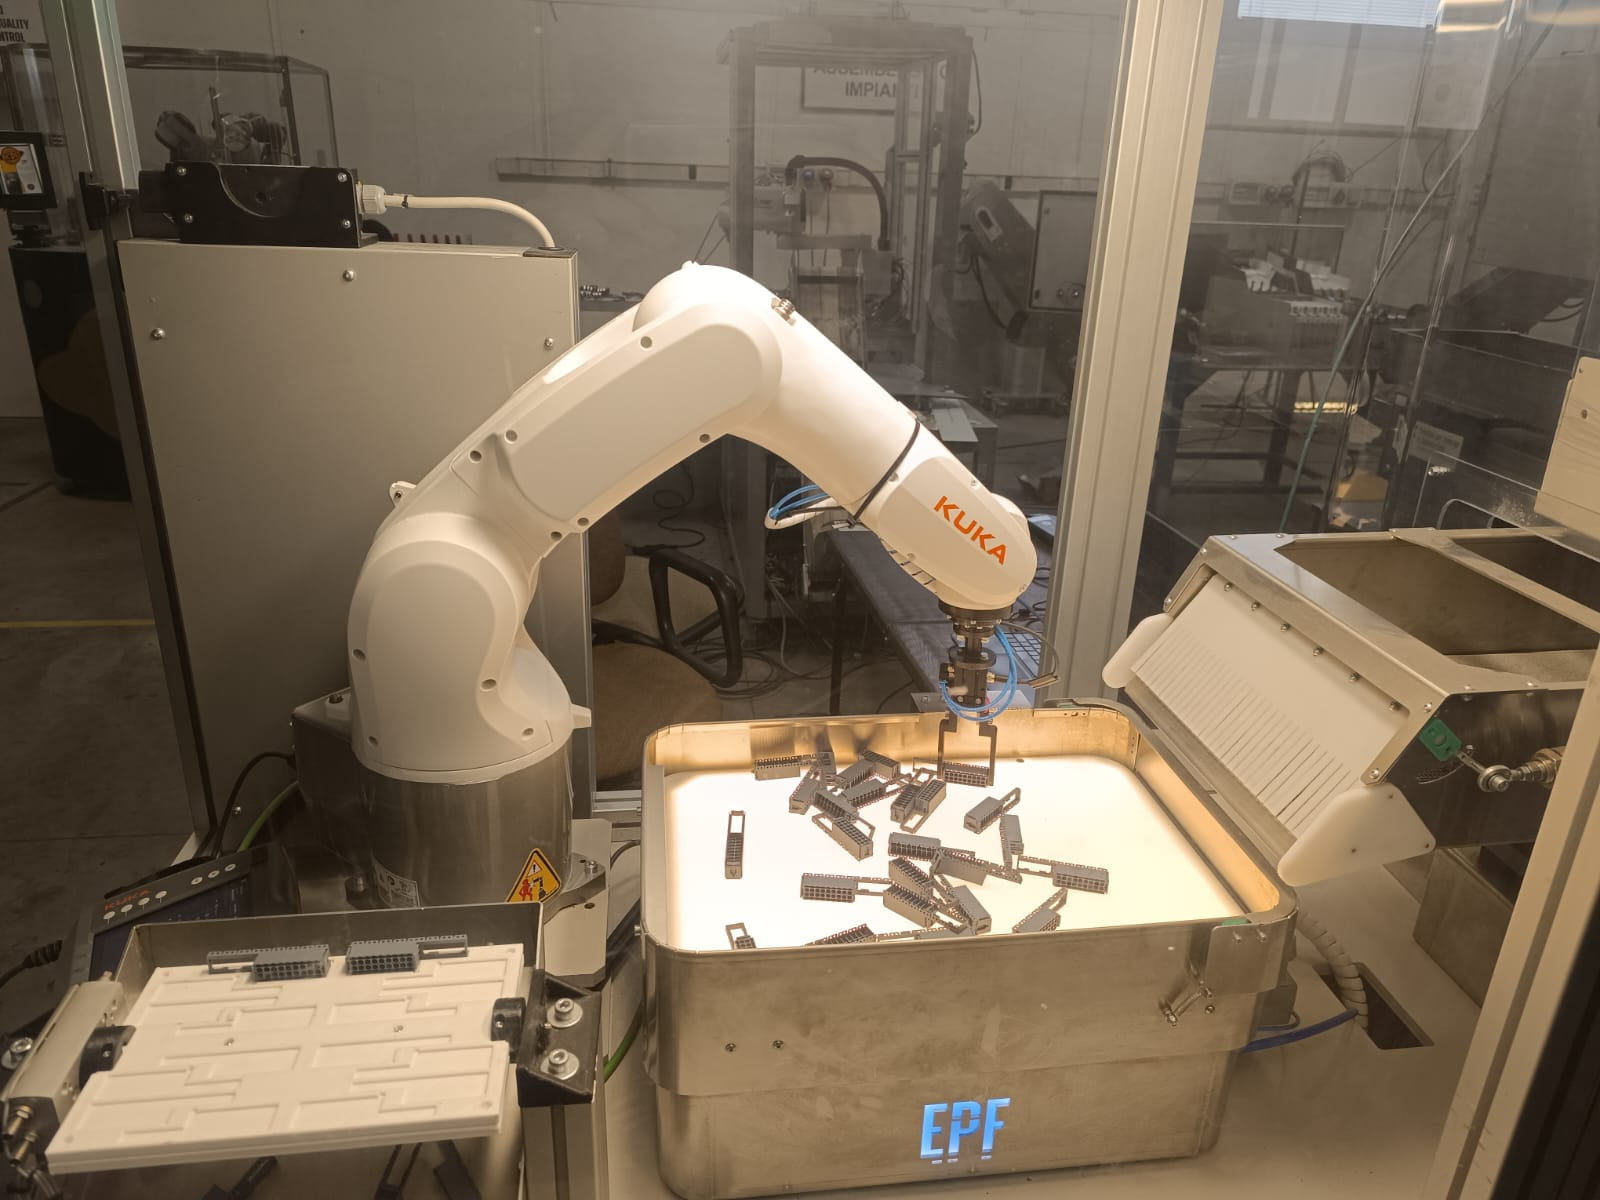
\includegraphics[width=0.8\textwidth]{images/chapter5Images/supata_overview.png}
	\caption{Overview of the SUPATA industrial system used for deployment and validation of the developed calibration module.}
	\label{fig:supata_overview}
\end{figure}

Prior to the deployment of the proposed calibration procedure, the machine exhibited reduced picking reliability, particularly for components located near the boundaries of the camera field of view. Subsequent analysis indicated that the issue originated primarily from inaccuracies in the intrinsic camera calibration. Due to the significant lens distortion present in the imaging system, even small calibration errors produced noticeable positional deviations in peripheral image regions, leading to degraded grasp accuracy.

To address this issue, a new calibration module was developed entirely in Python and integrated into the existing software environment used by the machine. The implemented solution employs a Chessboard-based calibration procedure and follows the same fundamental computer vision principles described throughout this thesis. Compared to the eye-in-hand calibration system investigated in the experimental campaign, the industrial application benefits from a simpler eye-to-hand geometry, since the camera remains fixed with respect to the workspace and therefore does not require estimation of a camera-to-end-effector transformation.

\begin{figure}[htbp]
	\centering
	
	% ------------------------------------------------
	% Original image with detected component
	% ------------------------------------------------
	\begin{subfigure}[t]{0.48\textwidth}
		\centering
		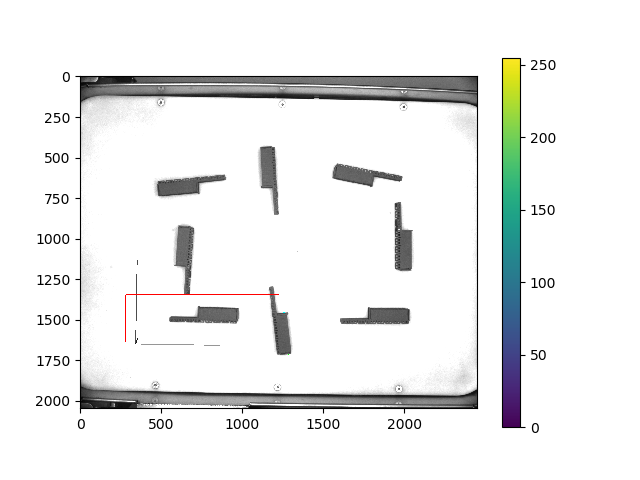
\includegraphics[width=\textwidth]{images/chapter5Images/supata_detection.png}
		\caption{Acquired image of the vibrating tray. The component selected for picking is highlighted by a red bounding box.}
		\label{fig:supata_detection_original}
	\end{subfigure}
	\hfill
	
	% ------------------------------------------------
	% Segmentation mask with grasp points
	% ------------------------------------------------
	\begin{subfigure}[t]{0.48\textwidth}
		\centering
		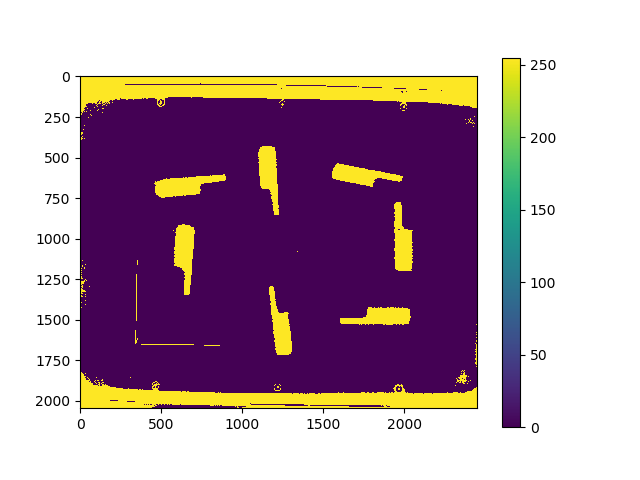
\includegraphics[width=\textwidth]{images/chapter5Images/supata_mask.png}
		\caption{Segmentation mask generated by the vision system masking out the selected component.}
		\label{fig:supata_detection_mask}
	\end{subfigure}
	
	\vspace{0.5cm}
	
	% ------------------------------------------------
	% Zoomed detail
	% ------------------------------------------------
	\begin{subfigure}[t]{0.70\textwidth}
		\centering
		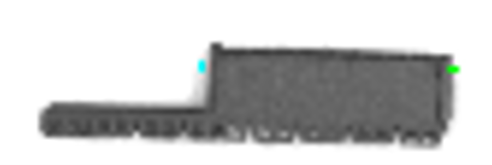
\includegraphics[width=\textwidth]{images/chapter5Images/supata_grasp_detail.png}
		\caption{Enlarged view of a single component showing the grasp reference points used to compute the robot picking pose.}
		\label{fig:supata_detection_detail}
	\end{subfigure}
	
	\caption{Vision-guided picking pipeline deployed on the industrial SUPATA system. The detected component is first identified within the tray, then segmented to extract the grasping features. The resulting image coordinates are transformed into robot coordinates using the calibrated camera model, enabling automatic pick-and-place operations.}
	\label{fig:supata_detection}
\end{figure}

Following integration of the new calibration pipeline, the system was deployed on a production machine delivered to the end customer. Operational validation was performed under normal production conditions. The machine executed continuous pick-and-place operations for approximately three working days, corresponding to roughly 24 hours of cumulative operation. Considering the average cycle time of approximately 3-4 seconds per component, the deployment involved on the order of $2 \times 10^{4}$ successful picking cycles.

Although no dedicated metrological evaluation was performed, the system maintained stable operation throughout the validation period without requiring recalibration or corrective intervention. In particular, the degradation in picking reliability previously observed near the image boundaries was no longer evident during operation.

\begin{figure}[htbp]
	\centering
	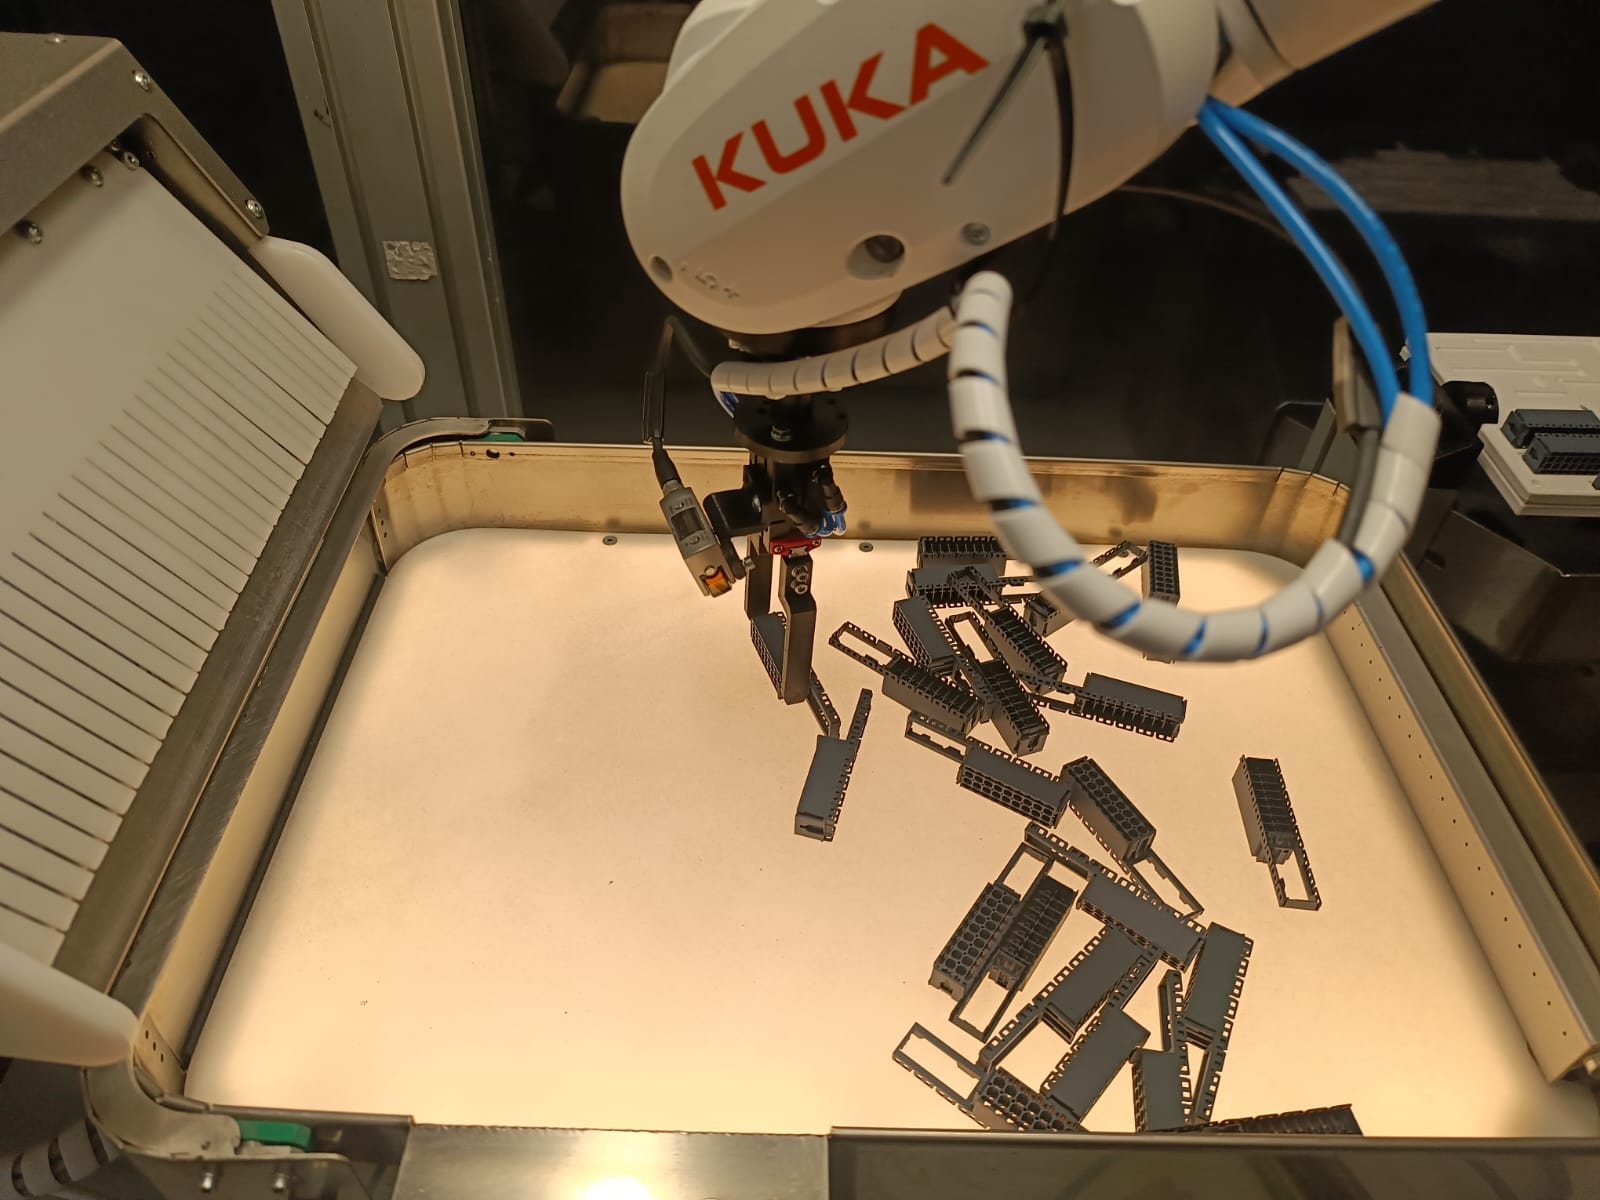
\includegraphics[width=0.8\textwidth]{images/chapter5Images/supata_tray_layout.png}
	\caption{Example of tray specification and placement layout used by the robotic system. The calibrated vision system enables accurate transformation of detected object positions into robot workspace coordinates.}
	\label{fig:supata_tray}
\end{figure}

The deployment demonstrates that the calibration methodology developed in this work is not limited to controlled laboratory experiments but can also be successfully applied within industrial production environments. While the validation does not provide a direct quantitative measurement of absolute positioning accuracy, the successful execution of a large number of production cycles without operational failures provides strong evidence of the practical effectiveness, robustness, and industrial applicability of the proposed calibration approach.




